\chapter{System Architecture}
\label{c:system}
Two major components in our system are: (a) processing of video frames using computer vision techniques to detect traffic lights, and (b) selection of a subpart of a frame using inertial sensor hints to reduce both computation time and spurious detection of traffic lights. 
In this chapter, we present the end-to-end system and describe various components of the system pipeline.

%% In this chapter, we discuss the system overview for traffic light detection.
%% This system detects the color of a traffic light in a recorded video frame.
%% We captured video using a smartphone along with the sensor data.

\section{Overview}
\label{s:overview}


\begin{figure}
\centering
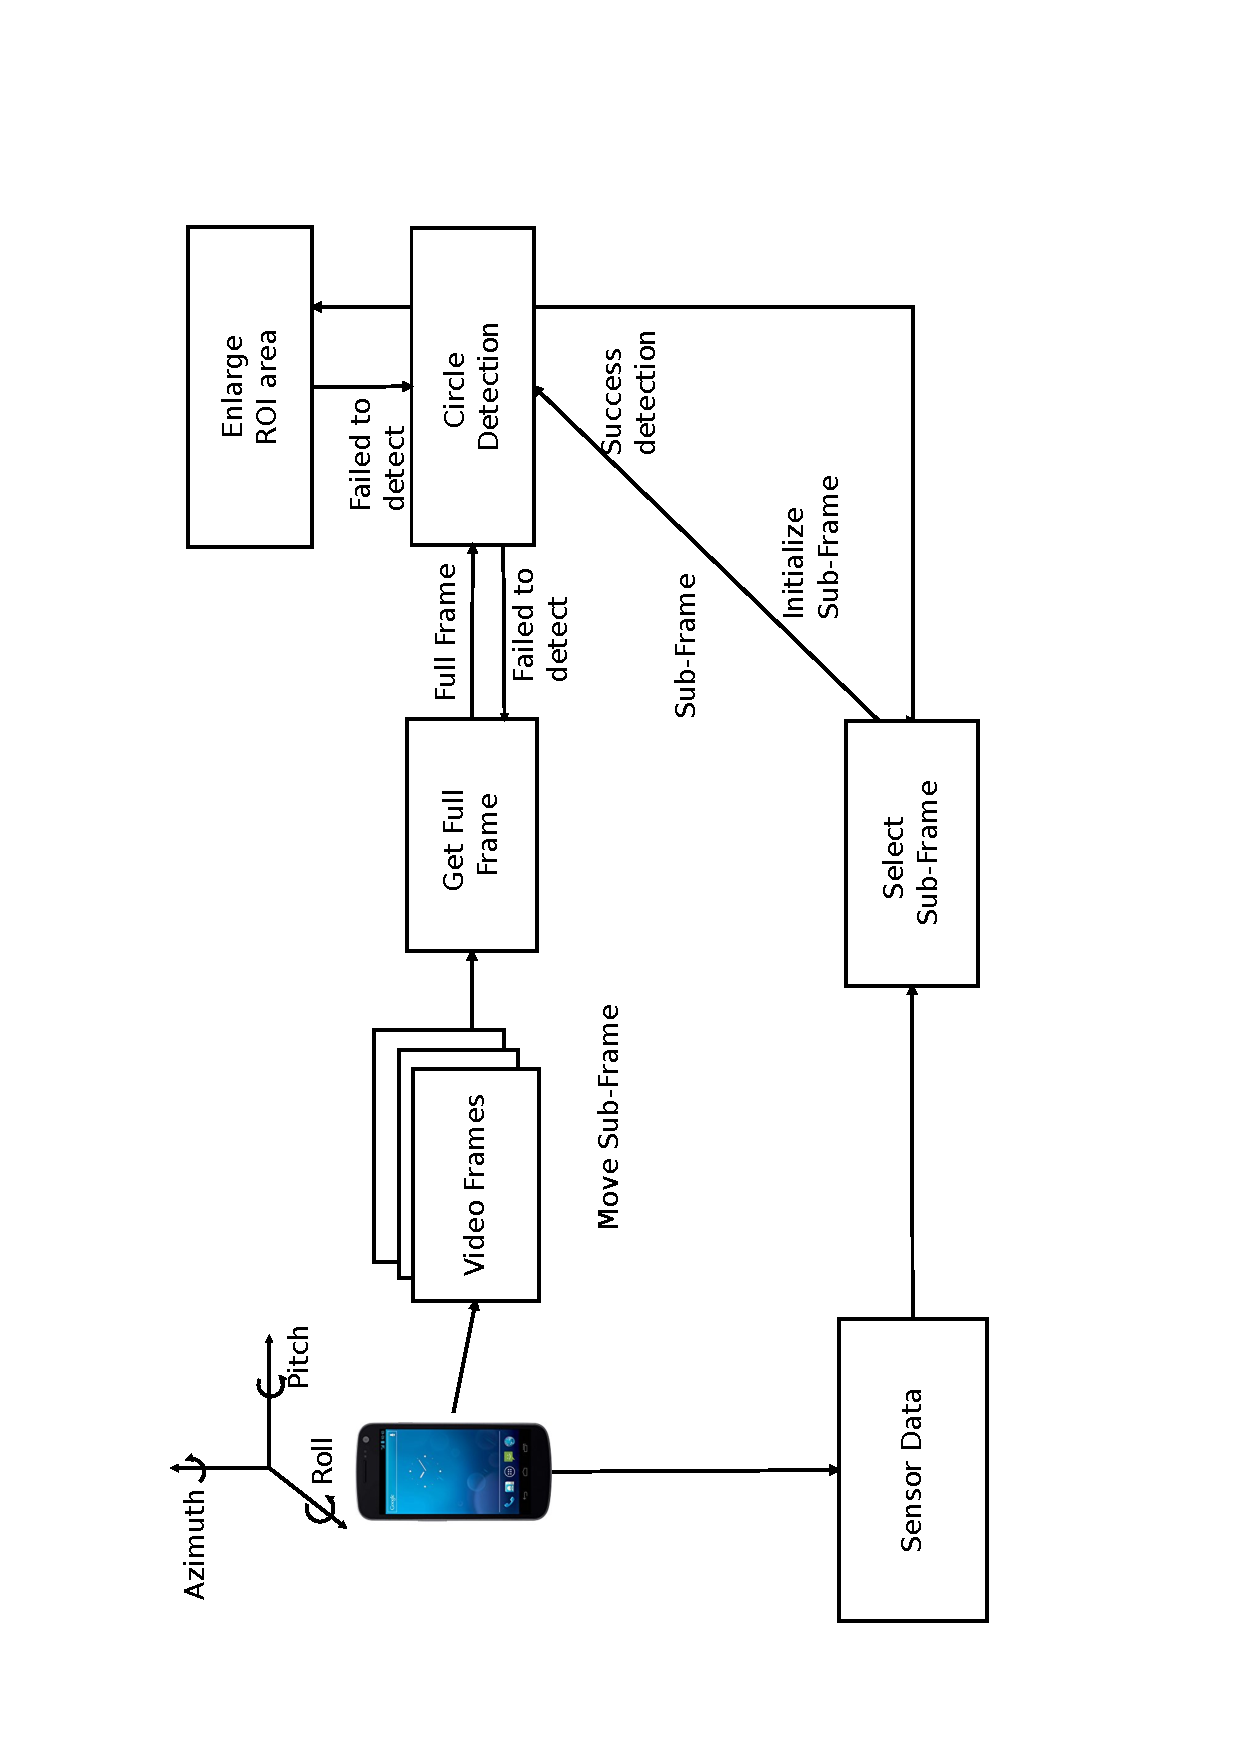
\includegraphics[width=5.2in]{figures/sysdia.pdf}
\caption{System Overview}
\label{f:sys_dia}
\end{figure}


Figure \ref{f:sys_dia} shows the overview of our system.
Using our smartphone app, we simultaneously record video and inertial sensor data.
Initially, we process the full region of the video frames to detect the traffic lights.
Once we successfully detect traffic lights in a video frame, we process only sub-parts of the subsequent frames using the sensor hints. 
For the subsequent frames, using the orientation change, we predict the region where the the traffic lights are likely to move and process only that region for detecting the traffic lights.
However, the prediction of region-of-interest (ROI) using the sensor hints can sometimes be incorrect.
In such cases, we gradually increase the area of the ROI until we detect traffic lights in that enlarged area. 
Note that the increment of the ROI can go up to the whole frame if there is no traffic lights in the frame or the traffic light detection algorithm fails to detect the existing traffic lights. 

The algorithm to detect traffic lights is same irrespective of processing of the full frame or a subpart of the frame.
Below, we discuss the the image processing algorithm for traffic light detection at first. 
Next, we discuss the procedure to select a subpart of a frame using sensor hints.


%We use three features of the traffic light, color, shape, and traffic bulb in a black box and the sensor feature of a smartphone as a system architecture for traffic light detection.
%% While recording the video we logged in the sensor data.
%% The first step of detection is the color filtering of the recorded videos.
%% Each video frames is consist of different colors.
%% In this step, each frame is filtered with only red and green pixel.
%% The traffic bulb shape is mostly circle.
%% To detect this characteristic we use Hough Circle  transformation\cite{hough_circle}.
%% Based on the traffic light detection position in video frames, we fix the region of interest area, which is a subpart of video frames.
%% After that, on next video frames the ROI change in respect to the sensor data. 


%% At first, we recorded videos along with the sensor data, gyroscope, accelerometer, pitch, roll, and azimuth.
%% These data have synchronization with our recorded video frames since we logged in sensor data while recording.
%% Now to detect the traffic light, we use three features of the traffic light.
%% Those are the color, shape of a traffic light and traffic light location in a black box.

\section{Image processing for traffic light detection}
The primary features of a traffic light is its bright red, yellow, or green color and the circular bulbs.
We use both these features for detecting the traffic lights. 
However, there can be other objects in the scene that can satisfy these properties such as circular red or green flower on people's clothing, red or green street signs etc.
To filter out such false detections, we use two heuristic filters, which utilize the fact that traffic lights are usually placed within a black box. 
Below, we discuss about these procedures in detail.

%% The first step of detection algorithm is color filtering of video frames.
%% Color filtering step filters out these candidate pixels from the video frames.


\subsection{Color space conversion}
The first step in our image processing pipeline is color space conversion.
We convert the BGR color space to HSV space.
To detect a specific color in BGR space, we need to use three different components (B, G, R).
However, HSV space has the property that we can detect a color based the single component, hue.
The range of hue values of each color are well defined and we utilze this range to keep the pixels of a desired color.


\subsection{Color filtering}
We only keep red and green pixels of a video frame for further processing in next stages.
In OpenCV \cite{opencv}, the hue range is from 0 to 180.
Table \ref{t:hue_range} shows the hue range for red and green colors.

\begin{table}[h!]
  \centering
  \caption{Hue range for red and green pixel.}
  \label{t:hue_range}
  \begin{tabular}{  l | c  }
    \hline
    Hue range for red & Lower 0 to 10 \\ \cline{2-2}
    & Upper 160 to 179 \\
    \hline \hline
    Hue range for green & 65 to 95 \\
    \hline
  \end{tabular}
\end{table}


\begin{figure*}[!ht]
\centering
\subfloat[Frame with red lights] {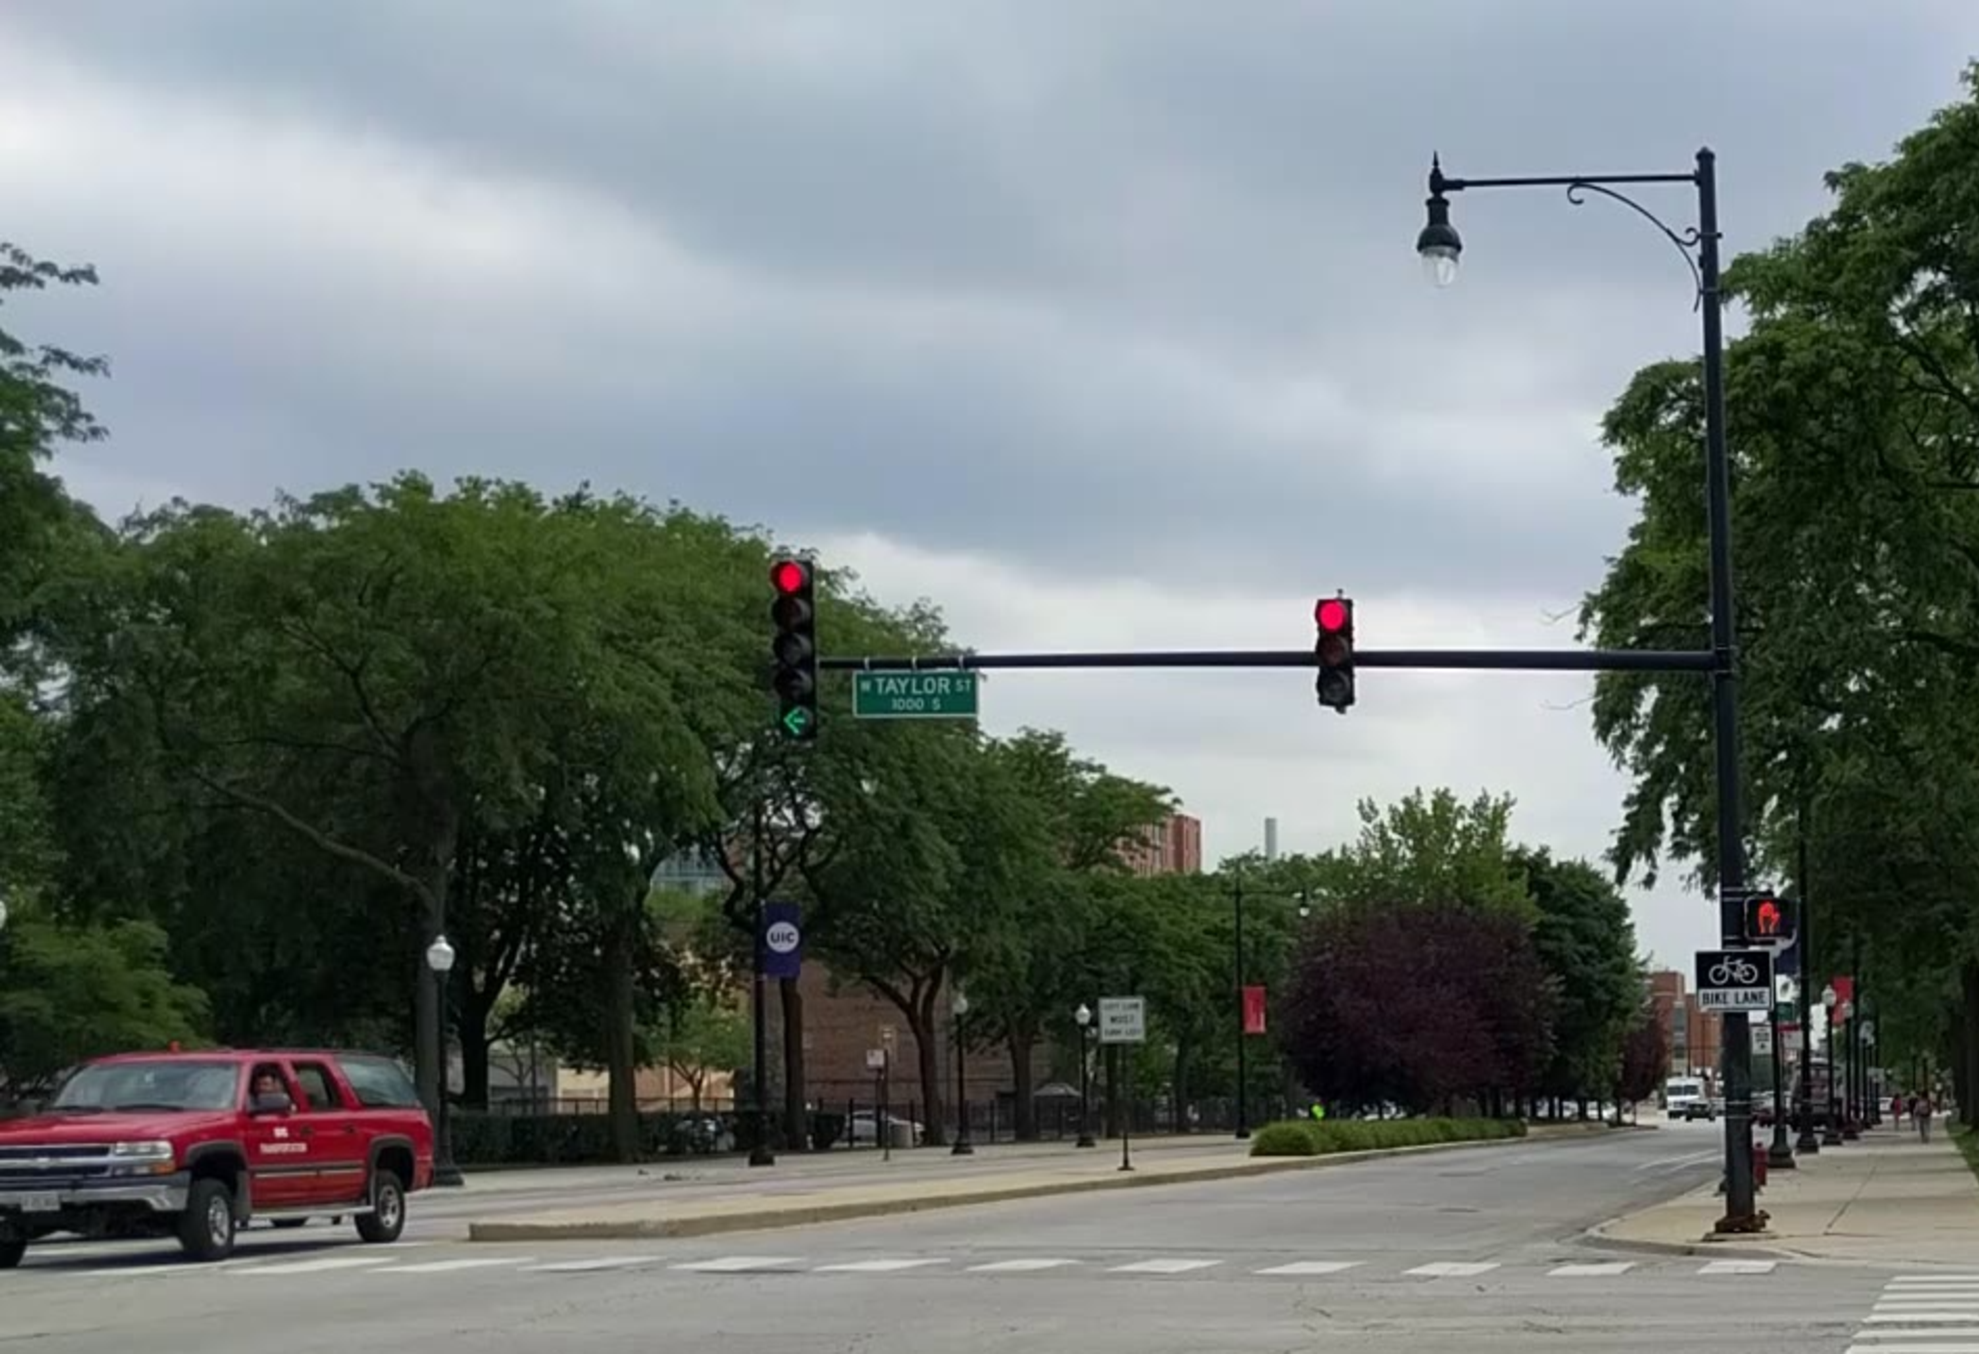
\includegraphics[width=3in]{images/frame301.pdf}}
\subfloat[Frame with green lights] {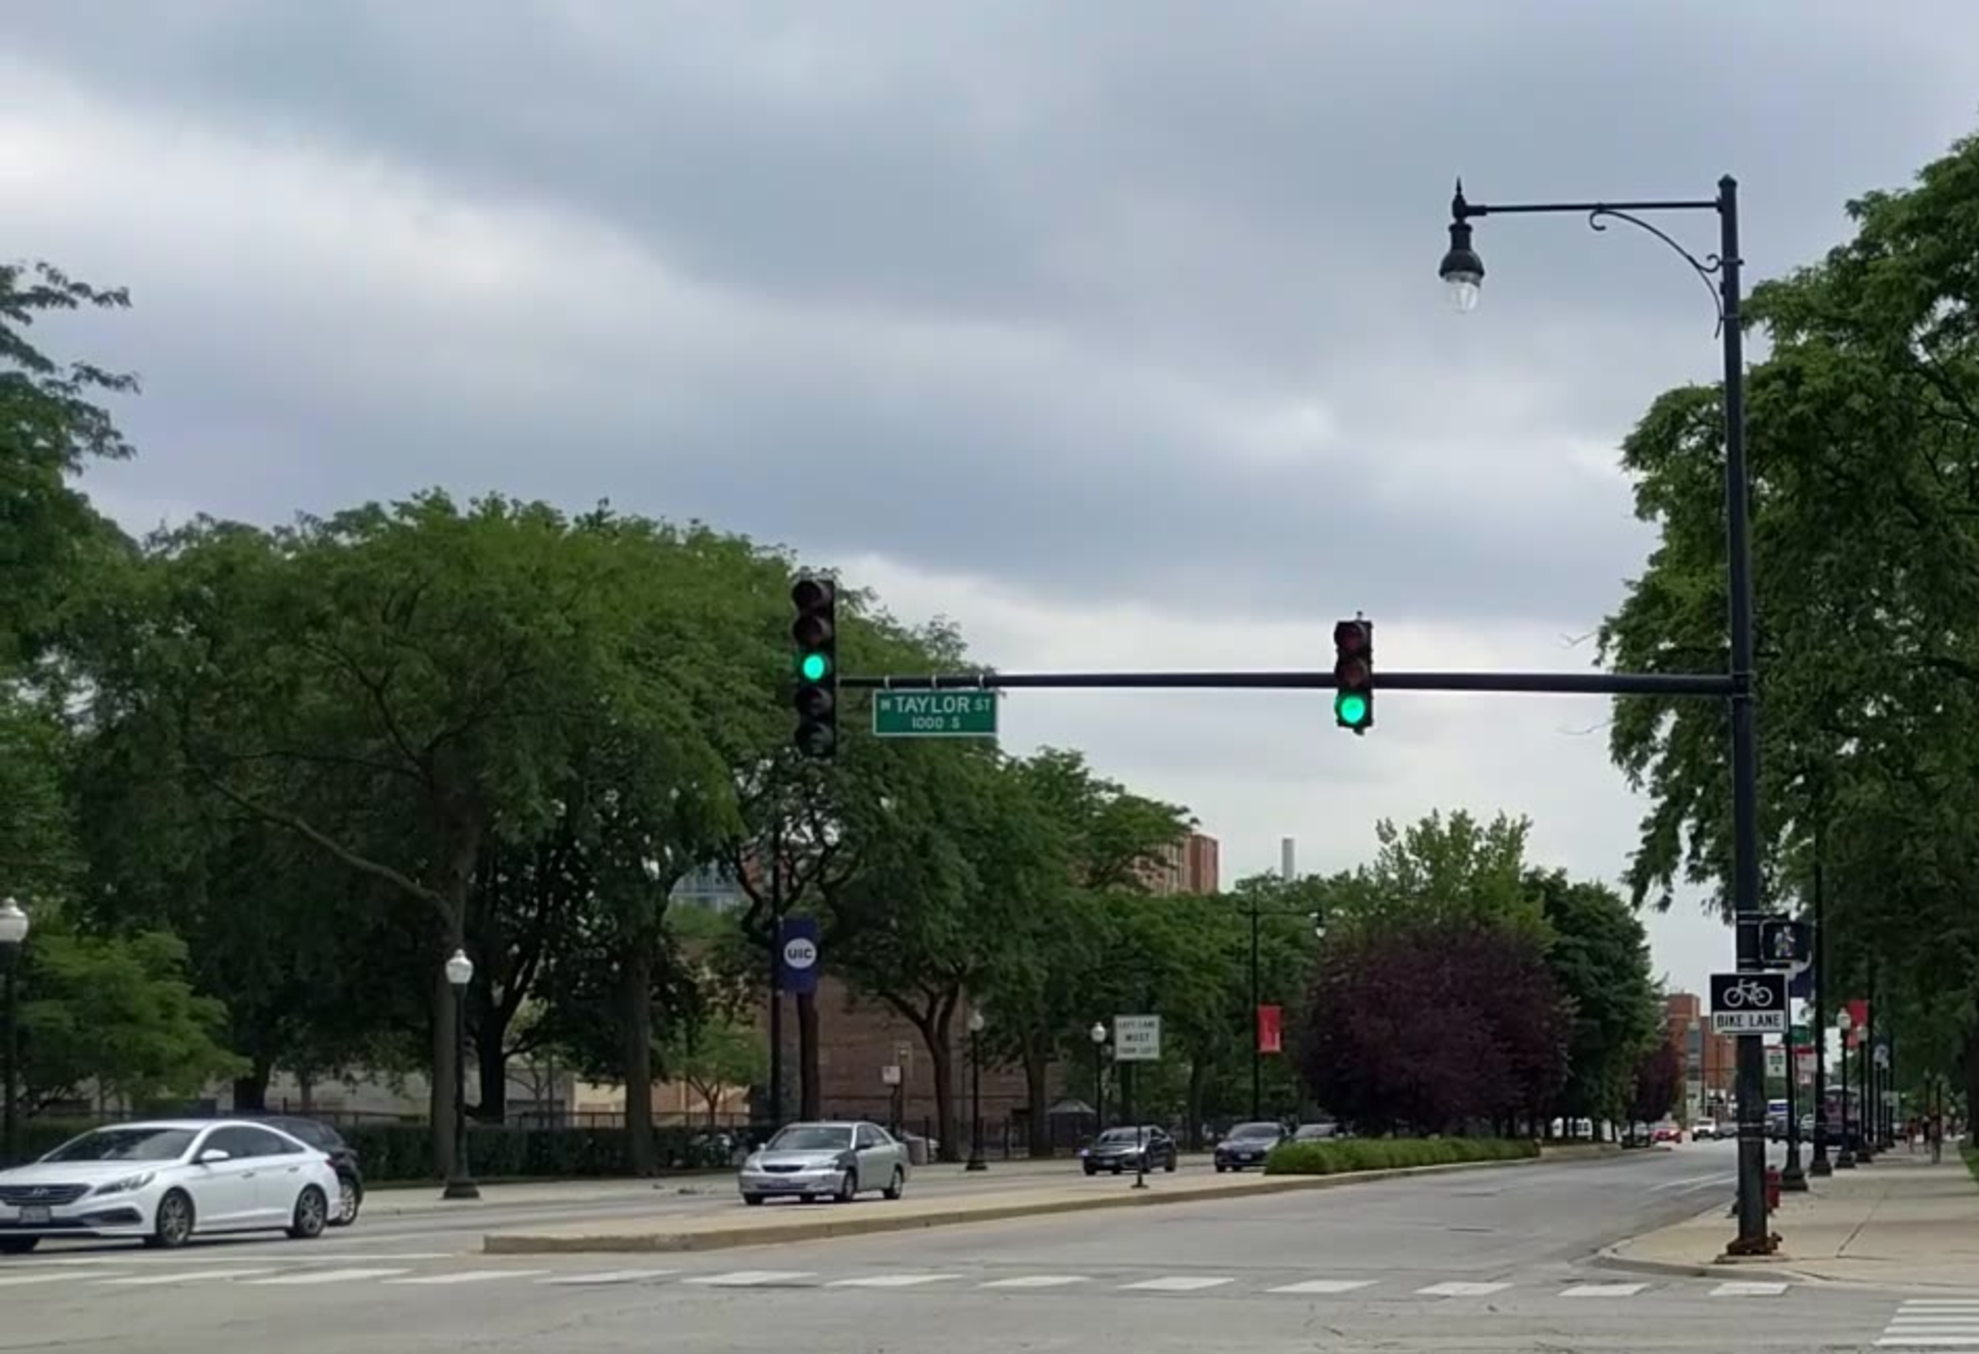
\includegraphics[width=3in]{images/frame502.pdf}}

\caption{Original videoframes.}
\label{f:org_img}
\end{figure*}

\begin{figure*}[!ht]
\centering
\subfloat[Frame with red lights] {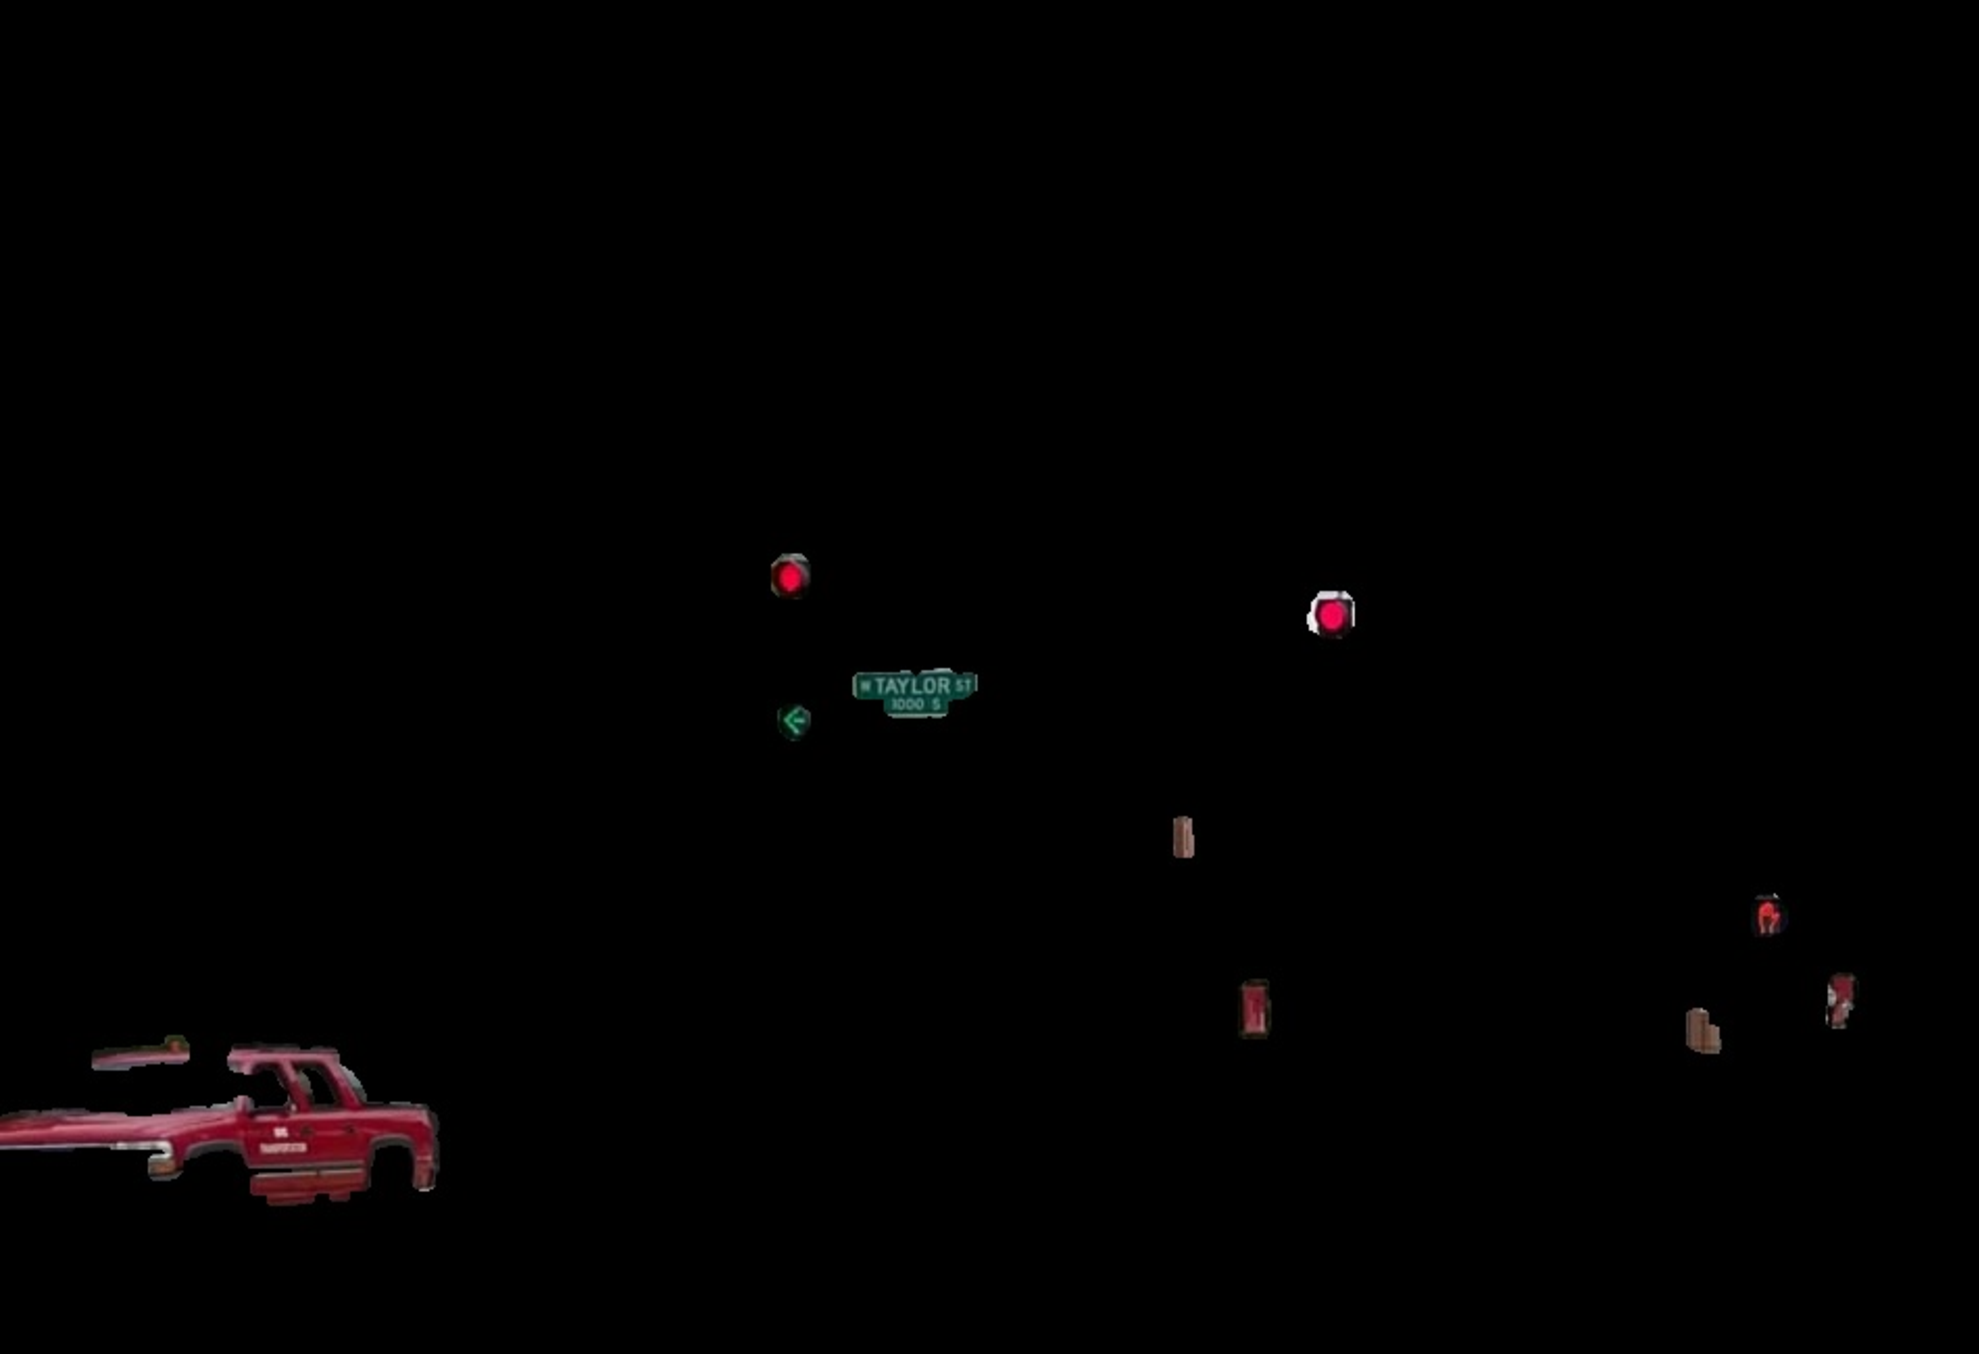
\includegraphics[width=3in]{images/RedGreenfiltering_red.pdf}}
\subfloat[Frame with green lights] {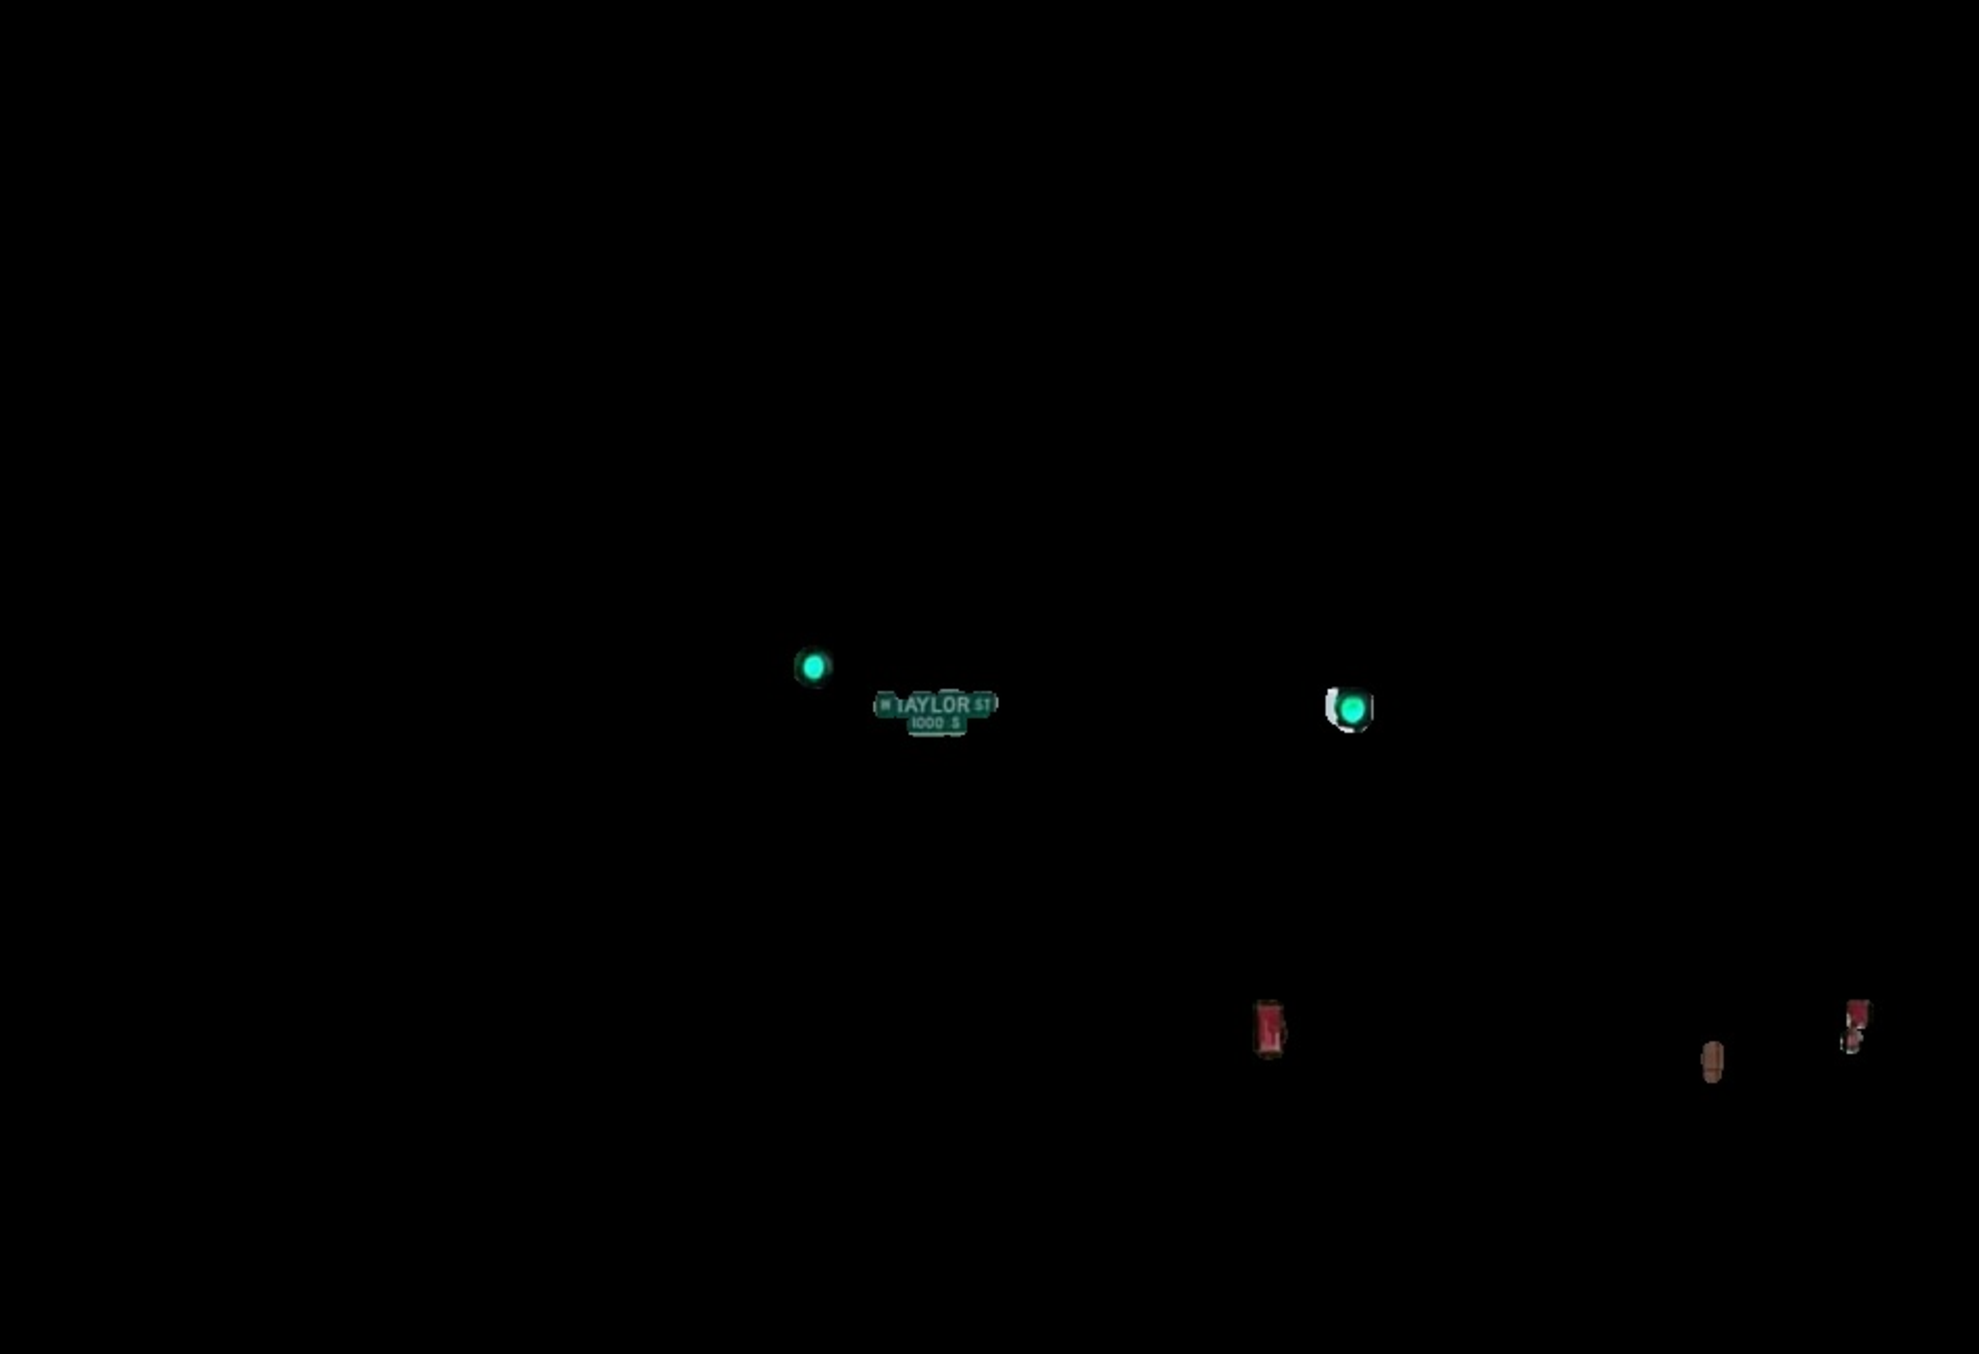
\includegraphics[width=3in]{images/RedGreenfiltering.pdf}}

\caption{Red green pixel filtering.}
\label{f:fil_img}
\end{figure*}

\ref{f:org_img}(a) shows the video frame with red traffic signal light and (b) shows the frame with green traffic signal light.
\ref{f:fil_img} shows the image with only red and green pixel.
(a) shows the filtering output with a red traffic light and (b) shows the filtering output with green traffic lights.
The color filtering process is computationally lightweight and it zeros out most of the pixels that reduce computational time to next steps.

\begin{figure}[h]
\centering
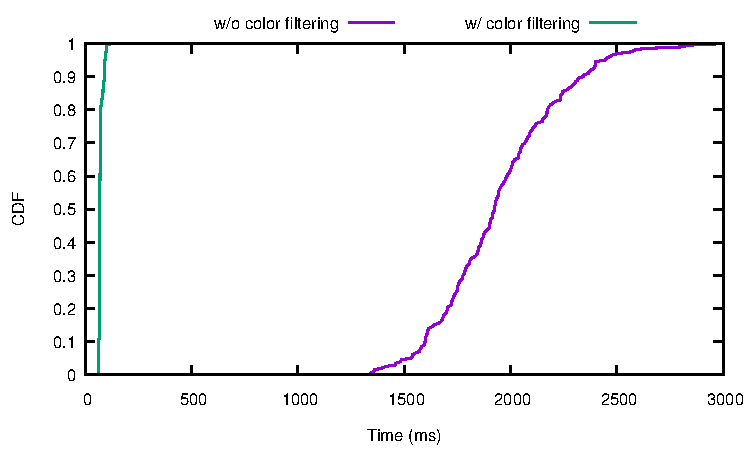
\includegraphics[width=5.2in]{plots/cdf_clrfil_full.pdf}
\caption{CDF for computational time comparison of the full videoframes with and without color filtering technique.}
\label{f:clrfil}
\end{figure}

\ref{f:clrfil} shows the computational time of the full videoframes with and without red and green color filtering technique.
It shows that color filtering process helps to reduce the processing time for all other steps significantly and this process itself is computationally lightweight.
\ref{f:clrfil} shows that the median of processing time is reducing from 2000 ms to 67 ms approximately. 

\subsection{Circularity check}
The next step of this detection algorithm is to detect the shape of traffic bulb (circle).
These filter images have only the desired pixel values.
To detect circle on this filtered images, we use Gaussian blur filter, in order to avoid false detection.
After this, we use the circle Hough Transform \cite{hough_circle} to detect the circles.
But, noise from the original images can fool the Hough transform to detect false and more circles.
As a solution to this problem, before converting our original BGR space frame to HSV space, a median filter is used.

\begin{figure*}[!ht]
\centering
\subfloat[Frame with red lights] {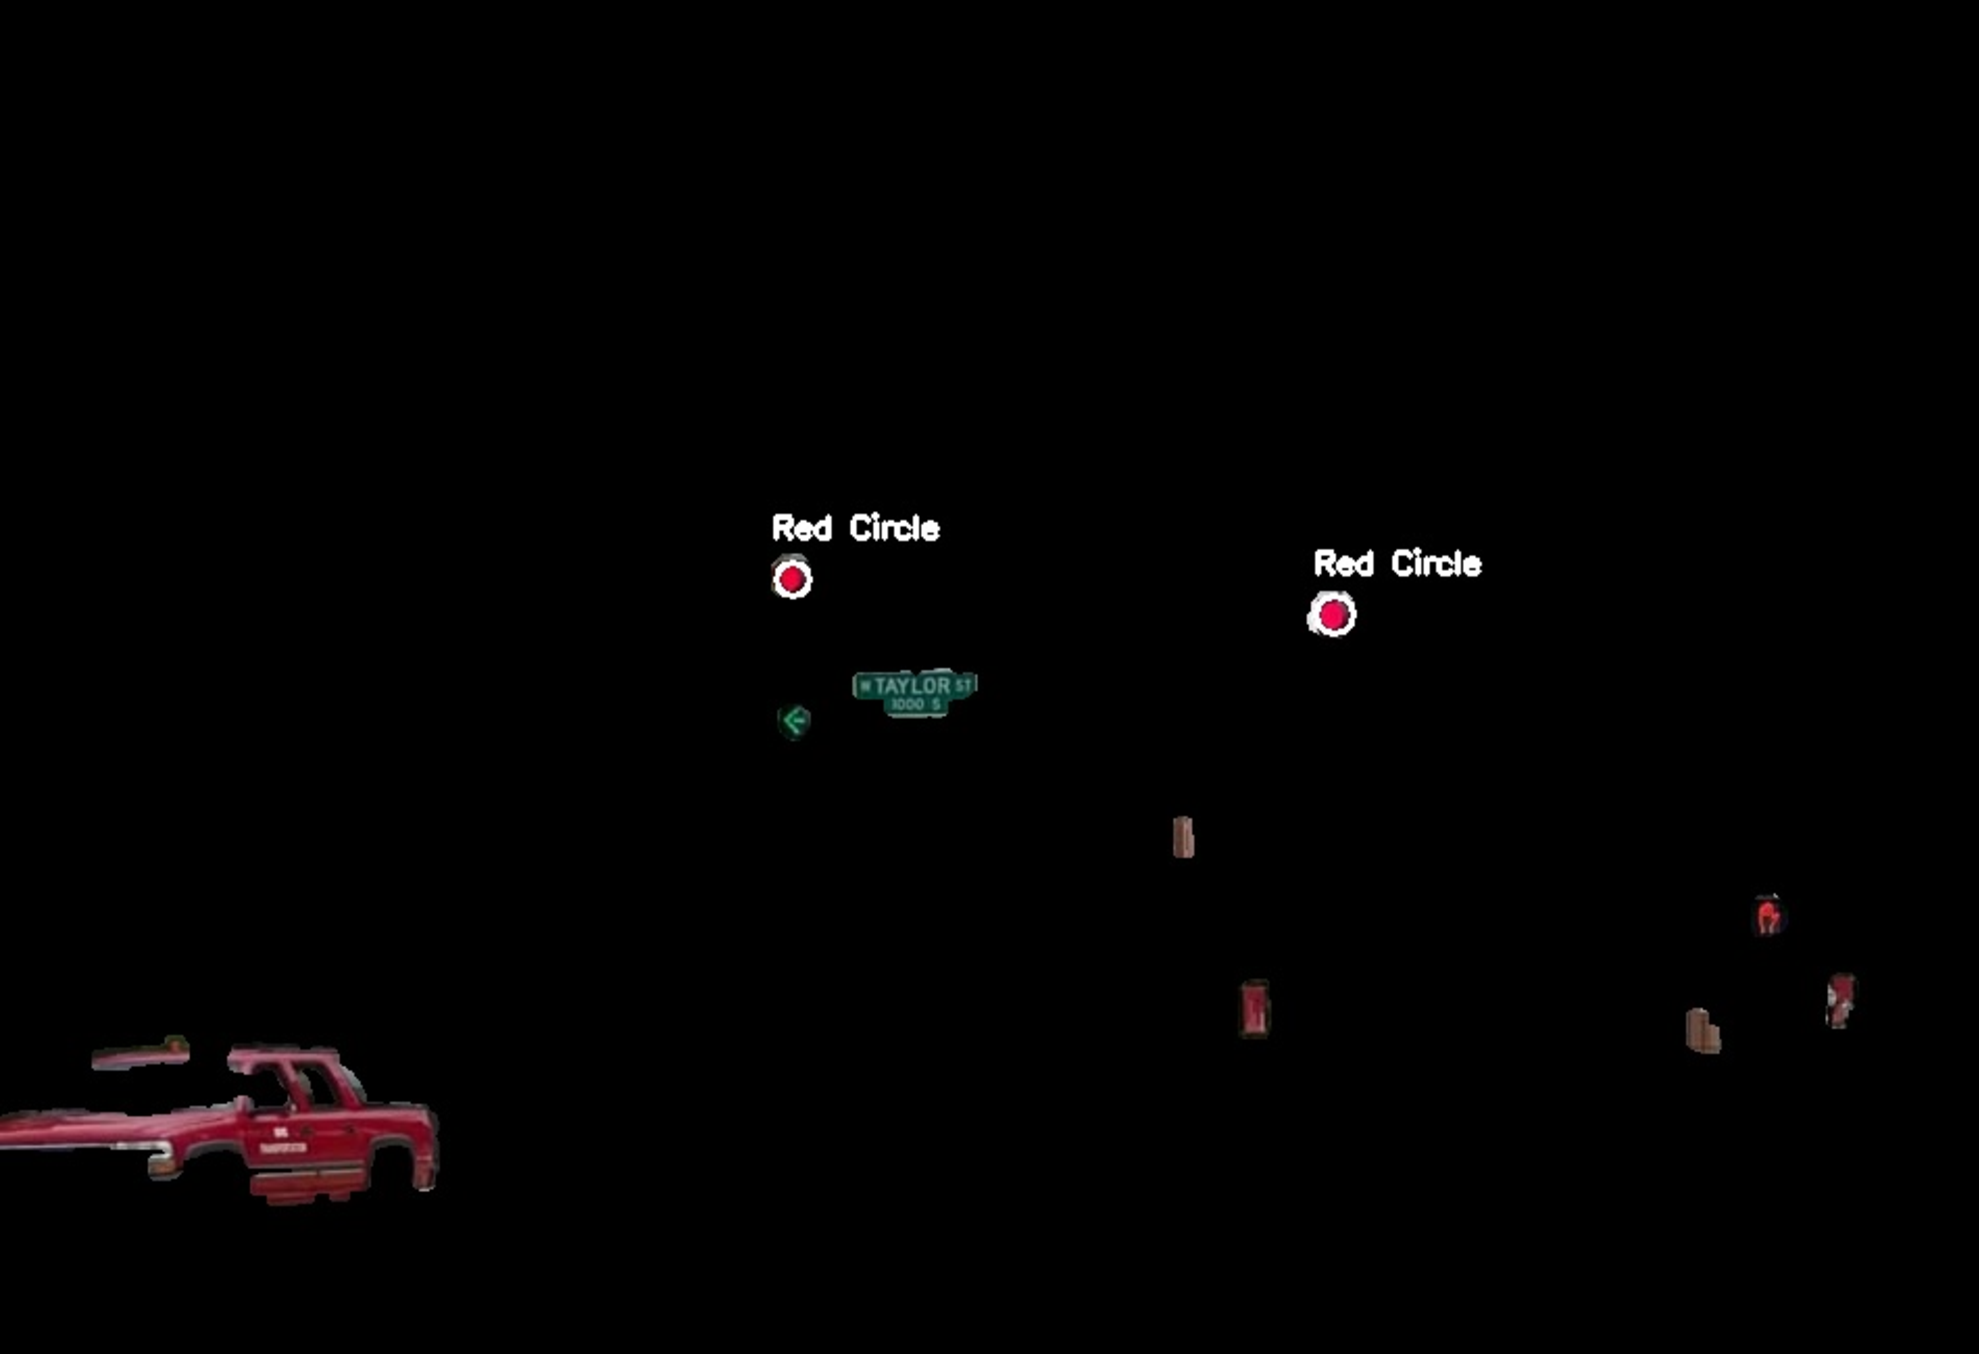
\includegraphics[width=3in]{images/Detectedredcircles.pdf}}
\subfloat[Frame with green lights] {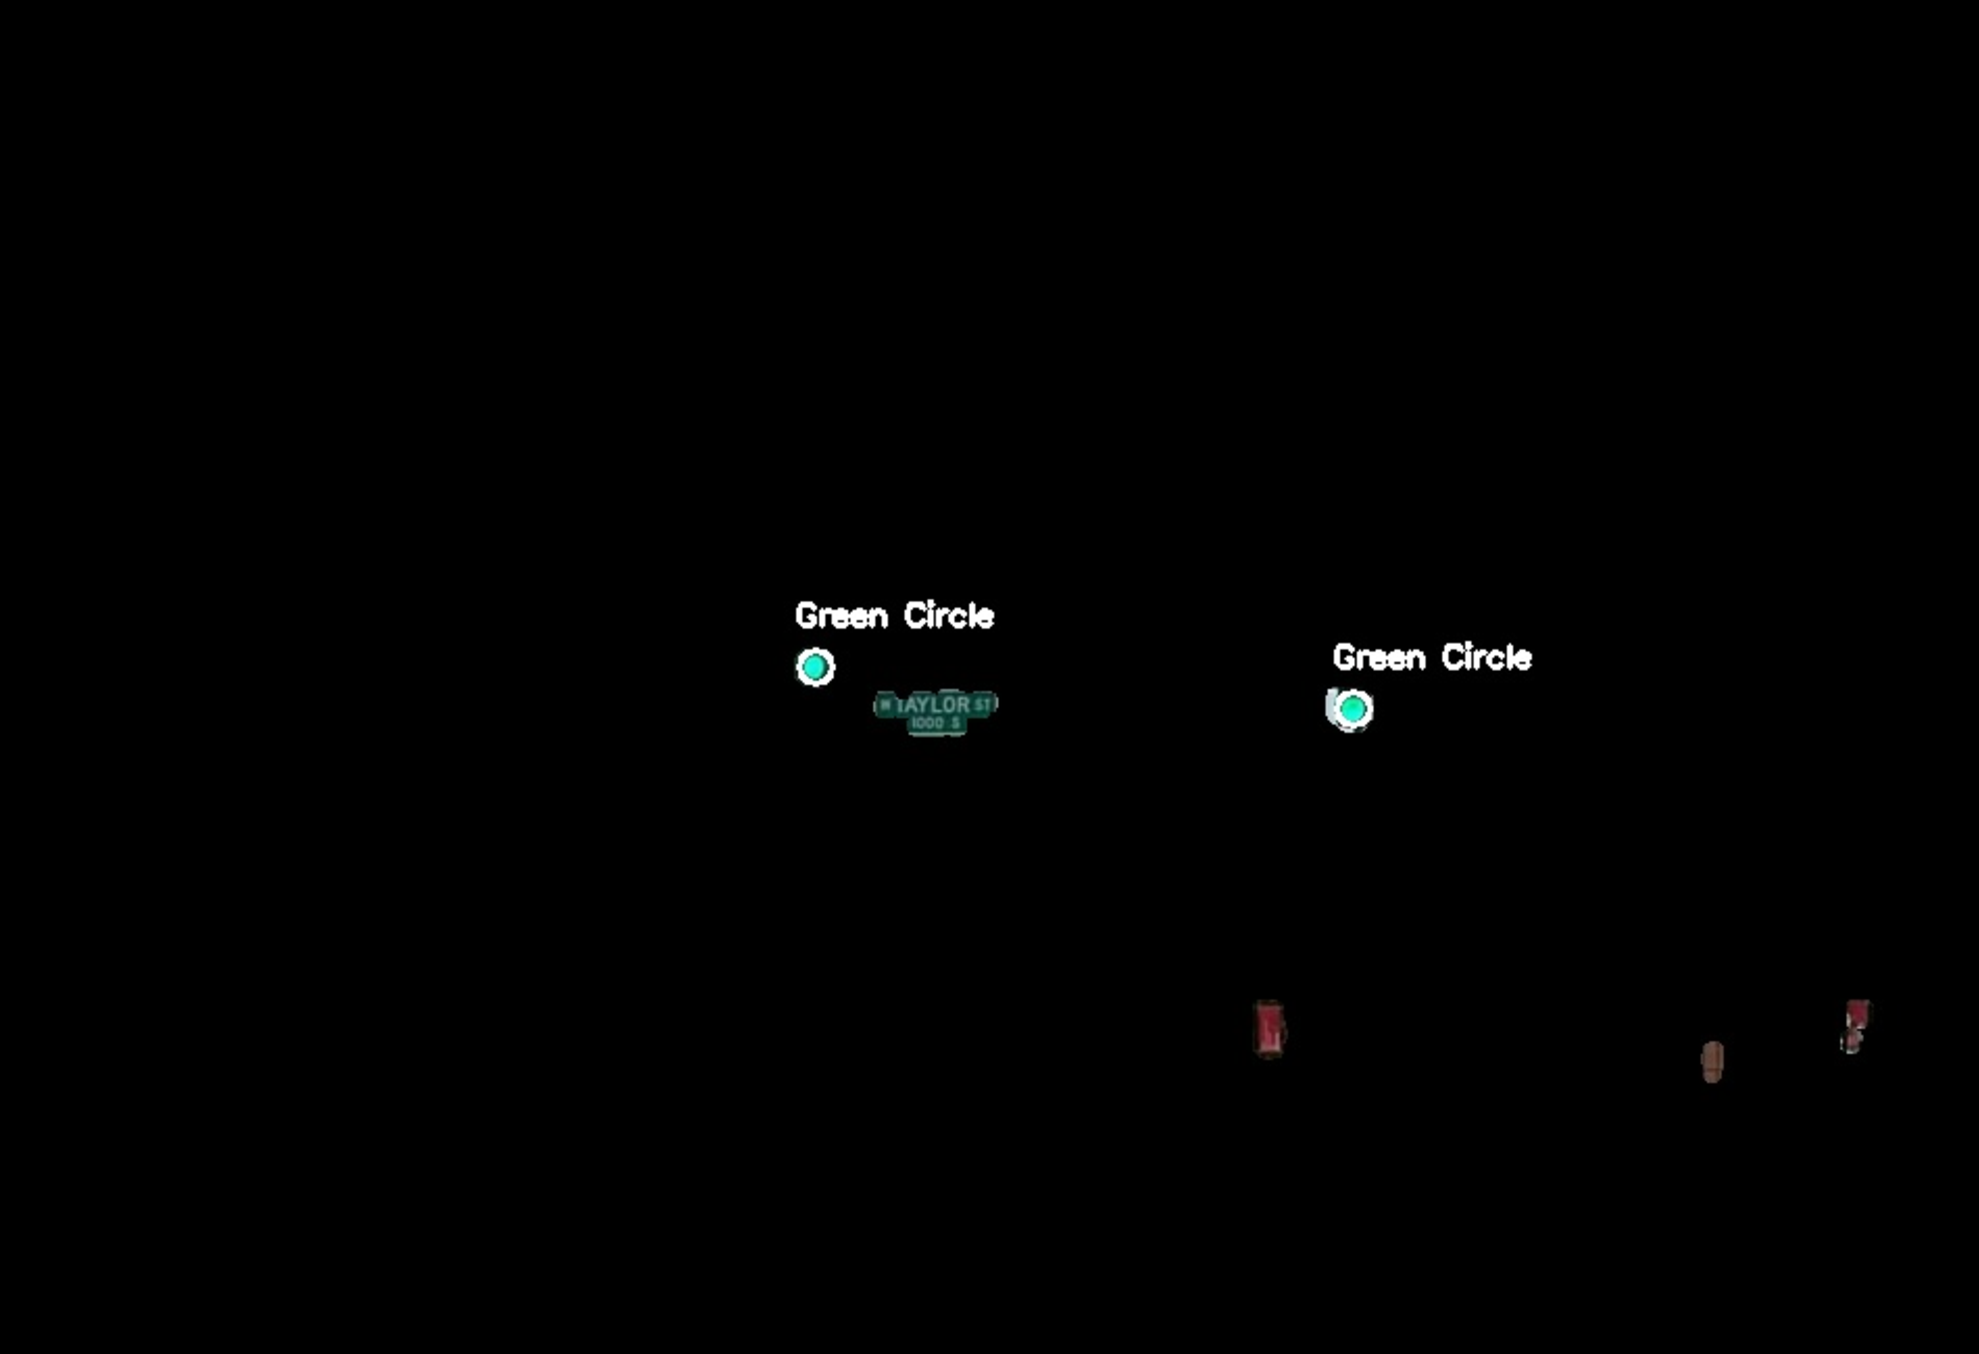
\includegraphics[width=3in]{images/Detectedgreencircles.pdf}}

\caption{Red green traffic bulb detection.}
\label{f:cir_img}
\end{figure*}

\ref{f:cir_img} shows the circle detection output.
(a) shows the red traffic light detection.
In this image, we have other red pixel values except for the traffic signal light.
But Hough circle transform can detect the circle precisely.
(b) shows the green traffic light detection output with Hough transform method.

\subsection{Heuristic filters}
\label{s:filter}
At this point, we have knowledge about the traffic bulb location and size (radius).
Now to detect if traffic bulb is in the black box, the other feature of our detection, we tried two heuristic filters.
Our first approach is to check pixels intensity of a circular area around the traffic bulb.
We use midpoint circle algorithm to find out the pixels value on a circular perimeter which is larger than our traffic bulb size.
our system gives a matrix with the count of pixels which has the intensity of a black color of all those points.
The intensity of black color can detect to check the Value of HSV space.
For black color, the range of the Value is very low, less than 40-45.
If this count is greater than our threshold we select that circle as our traffic bulb.
But we face some false detection problem with this approach.
Since the intensity of traffic bulb color is high and it spreads out also.
So we can not get a successful result with this approach.

\begin{figure*}[ht]
\centering
\subfloat[Red traffic bulb] {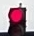
\includegraphics[width=2.2in]{images/redlight.jpg}}
\hfill
\subfloat[Green traffic bulb] {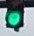
\includegraphics[width=2.2in]{images/greenlight.jpg}}\\

\caption{Red and green traffic bulb intensity.}
\label{f:bulb_int}
\end{figure*}

\ref{f:bulb_int} shows the red and green traffic bulb intensity.
We can see that the color spreads out around the exact circle area.
So the black color intensity measurement around the bulb circle area using midpoint circle algorithm is not giving an actual result.

Our second approach is to scan a rectangle frame  around the traffic light.
Traffic bulbs locate in a black box, which can place in horizontally or vertically in street.
To make our approach more global we scan all around the traffic light to check the intensity.
Our system gives a matrix of the no of pixels that have the intensity same as black color.
If this pixel no is more than our threshold value we consider that the detected circle is in the traffic signal black box and we finally detect that circle as our traffic bulb.
\begin{figure}[!ht]
\centering
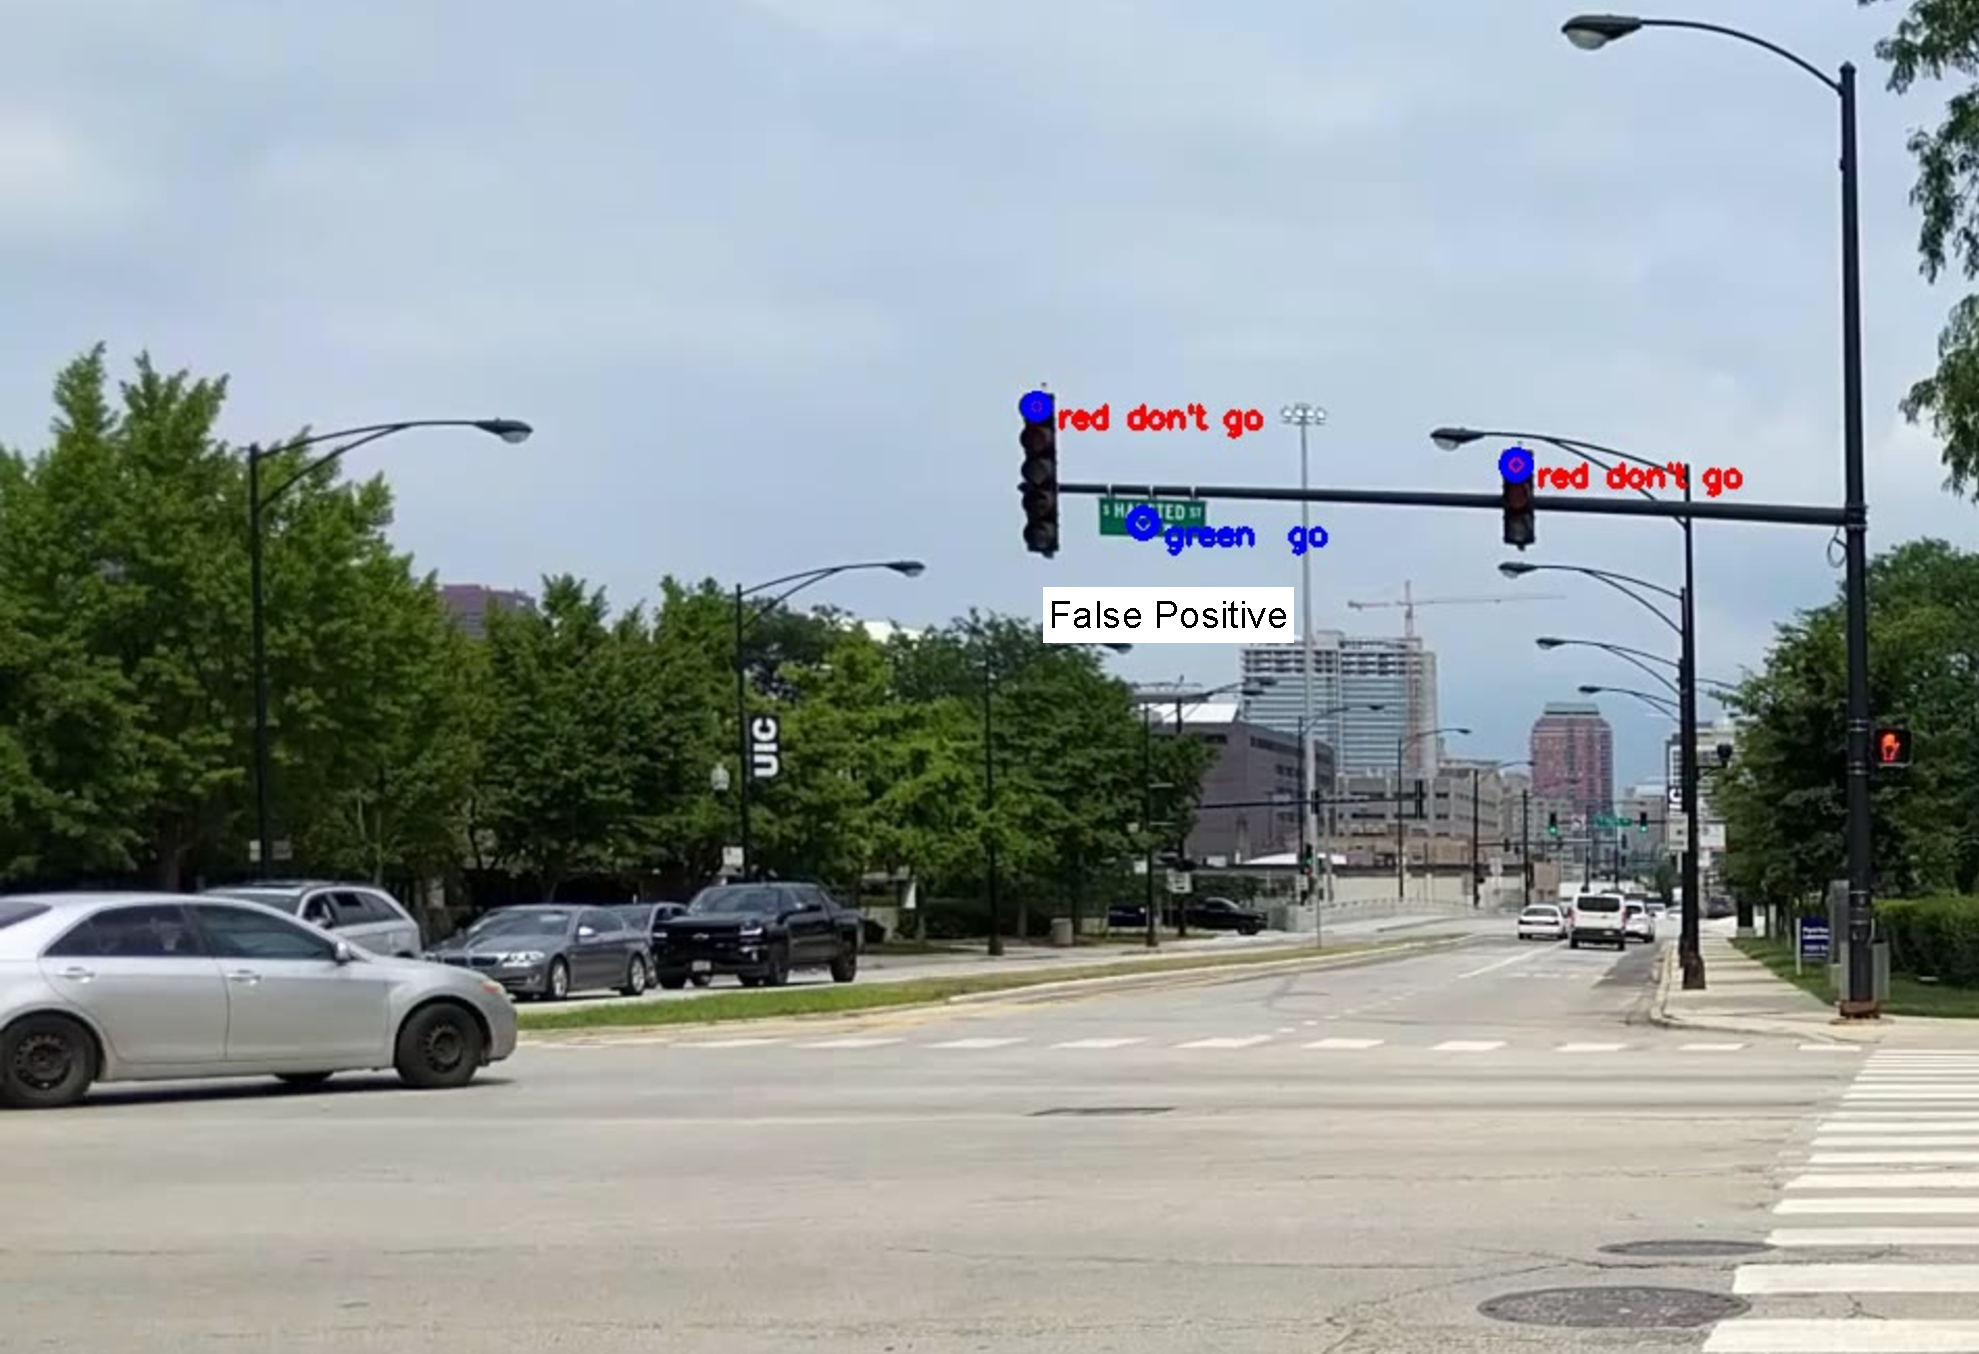
\includegraphics[width=4.2in]{images/norec_filter.pdf}
\caption{Output not using black box checking filter.}
\label{f:norec_filter}
\end{figure}

\ref{f:norec_filter} shows there is one green false positive between two red traffic light.
That false green circle actually a street nameplate and around that there is no black box.
So when we use our black box checking filter we can remove this false positive detection.
\ref{f:rec_filter} shows the output after using our heuristic black box checking filter.




\begin{figure}[ht!]
\centering
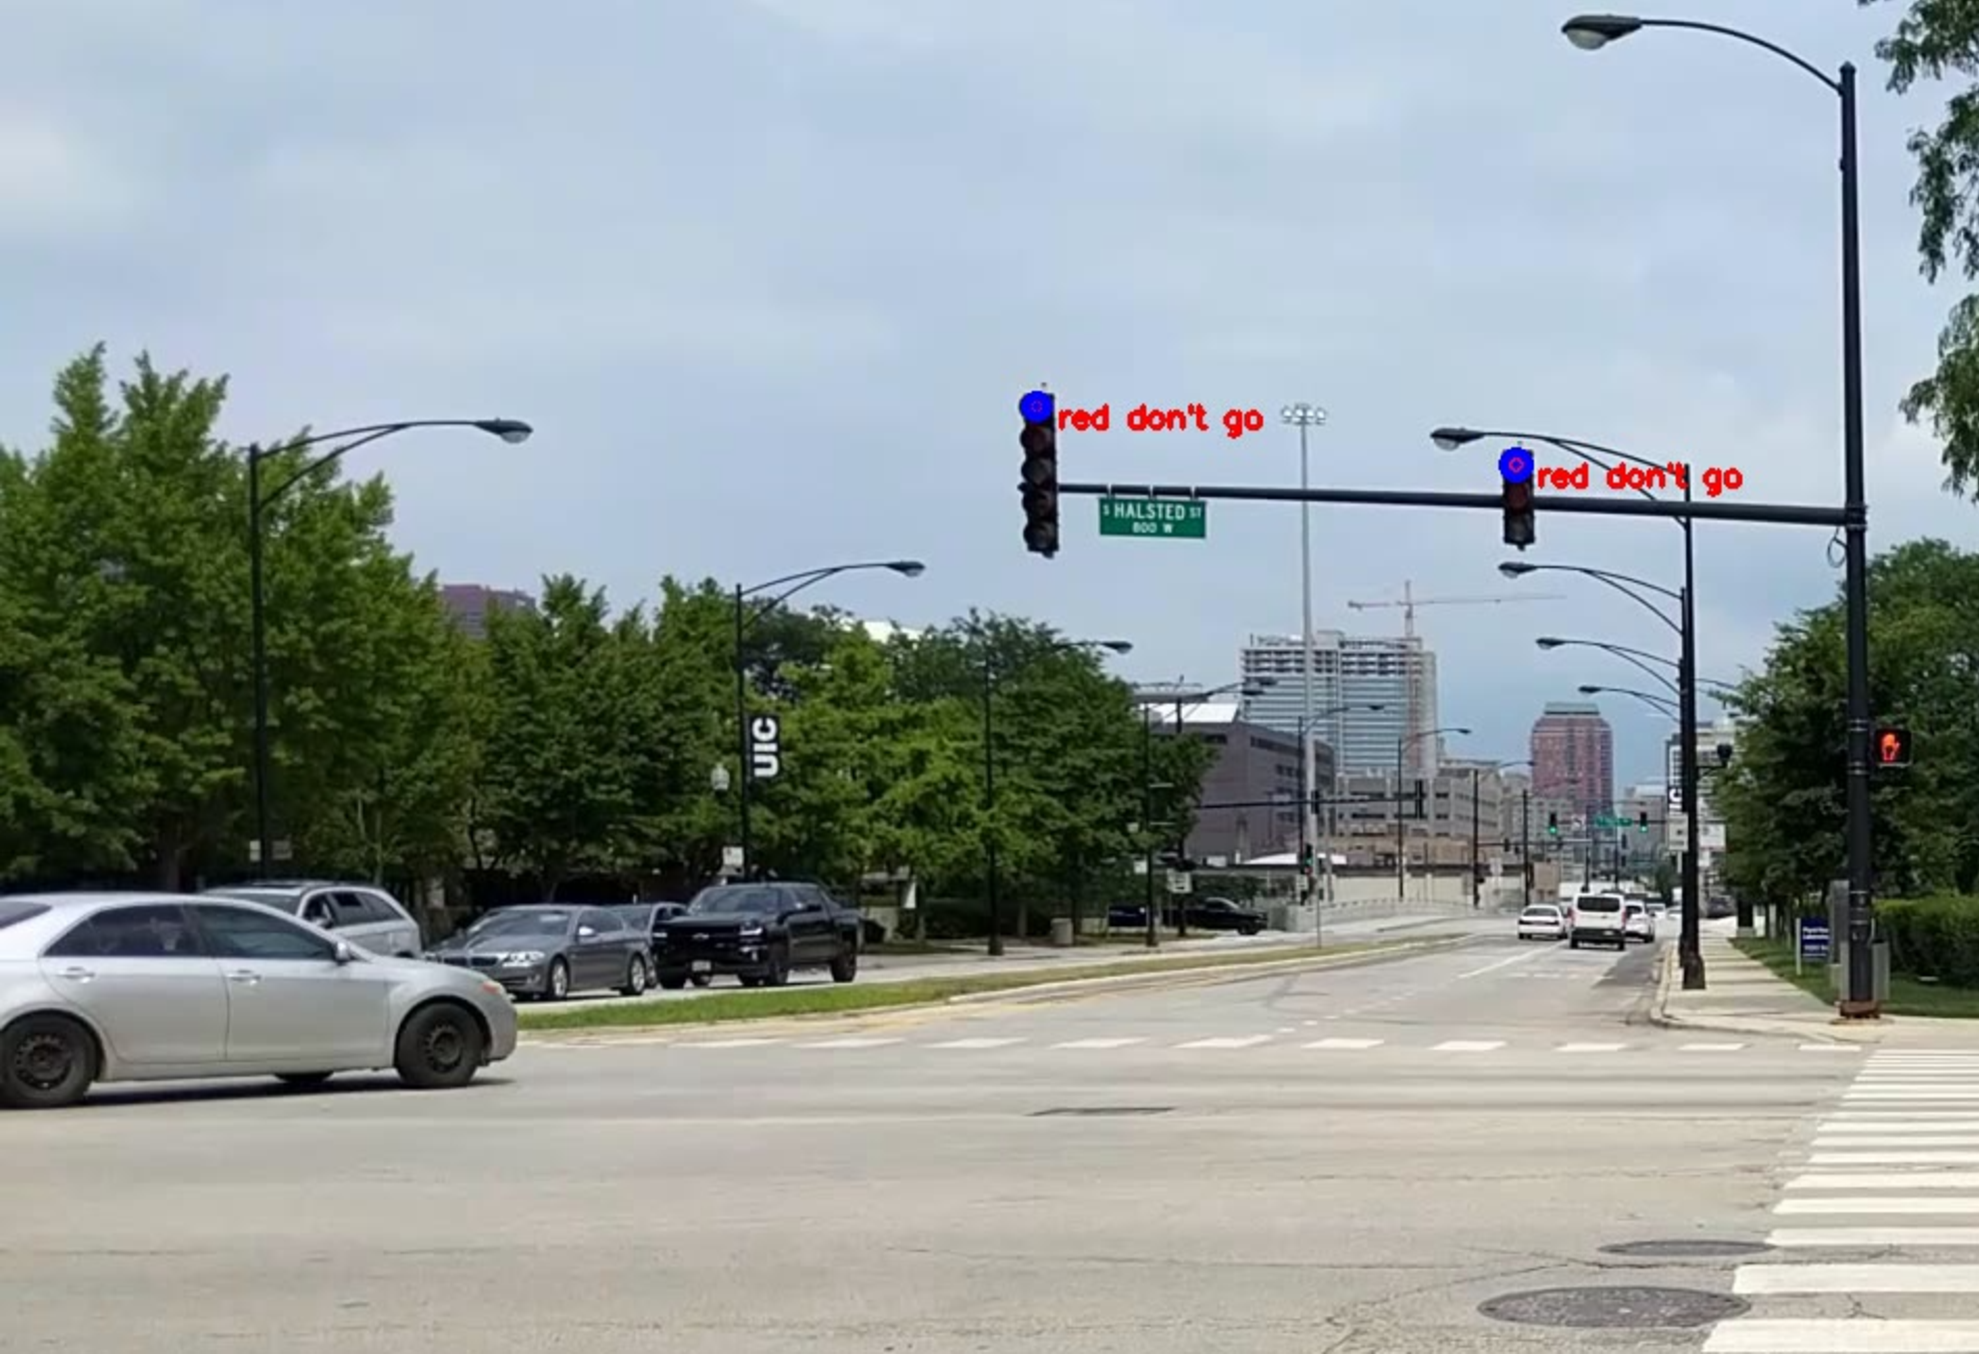
\includegraphics[width=4.2in]{images/rec_filter.pdf}
\caption{Output using black box checking filter.}
\label{f:rec_filter}
\end{figure}

\section{Sensor fusion for subpart selection}

\subsection{Synchronization of sensors and video frames}
To improve our detection we also use the smartphone's sensor data hints.
Our system logged the sensor data while recording the video.
From the logged data we know the time for sensor data registered.
We have the time when the video is recorded.
After that, we synchronized our data with the video using the starting time of the video and the frame rate.
So, using the frame rate and starting time we know the time for each frame, and from the logged sensor data, we know the sensor value corresponds to the time.
Using this time and our frame time we interpolated sensor hints if we miss any data corresponding to that frame.
Finally, we get the synchronized sensor data with our recorded video.

\ref{} shows the interface of our android app.
So when we start recording the pitch, roll and azimuth display in the screen and also start registering in a file.

\subsection{Region-Of-Interest selection}
\label{s:roi}
Now, when we detect a traffic light in our video frame successfully using the color, shape of the traffic light and the characteristics of traffic bulb being in a box, we have the idea of the position of the traffic light.
With this idea we subdivide our video frame making a region of interest area.
When we move to the next frame, we have a prior knowledge of traffic light position and we know the sensor data, pitch, roll, and azimuth of this frame.
Using these sensor data of the current frame and the previous frame we have the idea of the movement of the traffic light.
With this change of movement, the ROI also moves to the direction of change.
\ref{f:rec_mv}shows the movement of ROI with the change of pitch and azimuth of our recorded video.
Apart from this, when our system can not detect any circle in our specific ROI area, it updates the ROI and tries to detect the light.

\begin{figure*}[!ht]
\centering
\subfloat[Initial ROI] {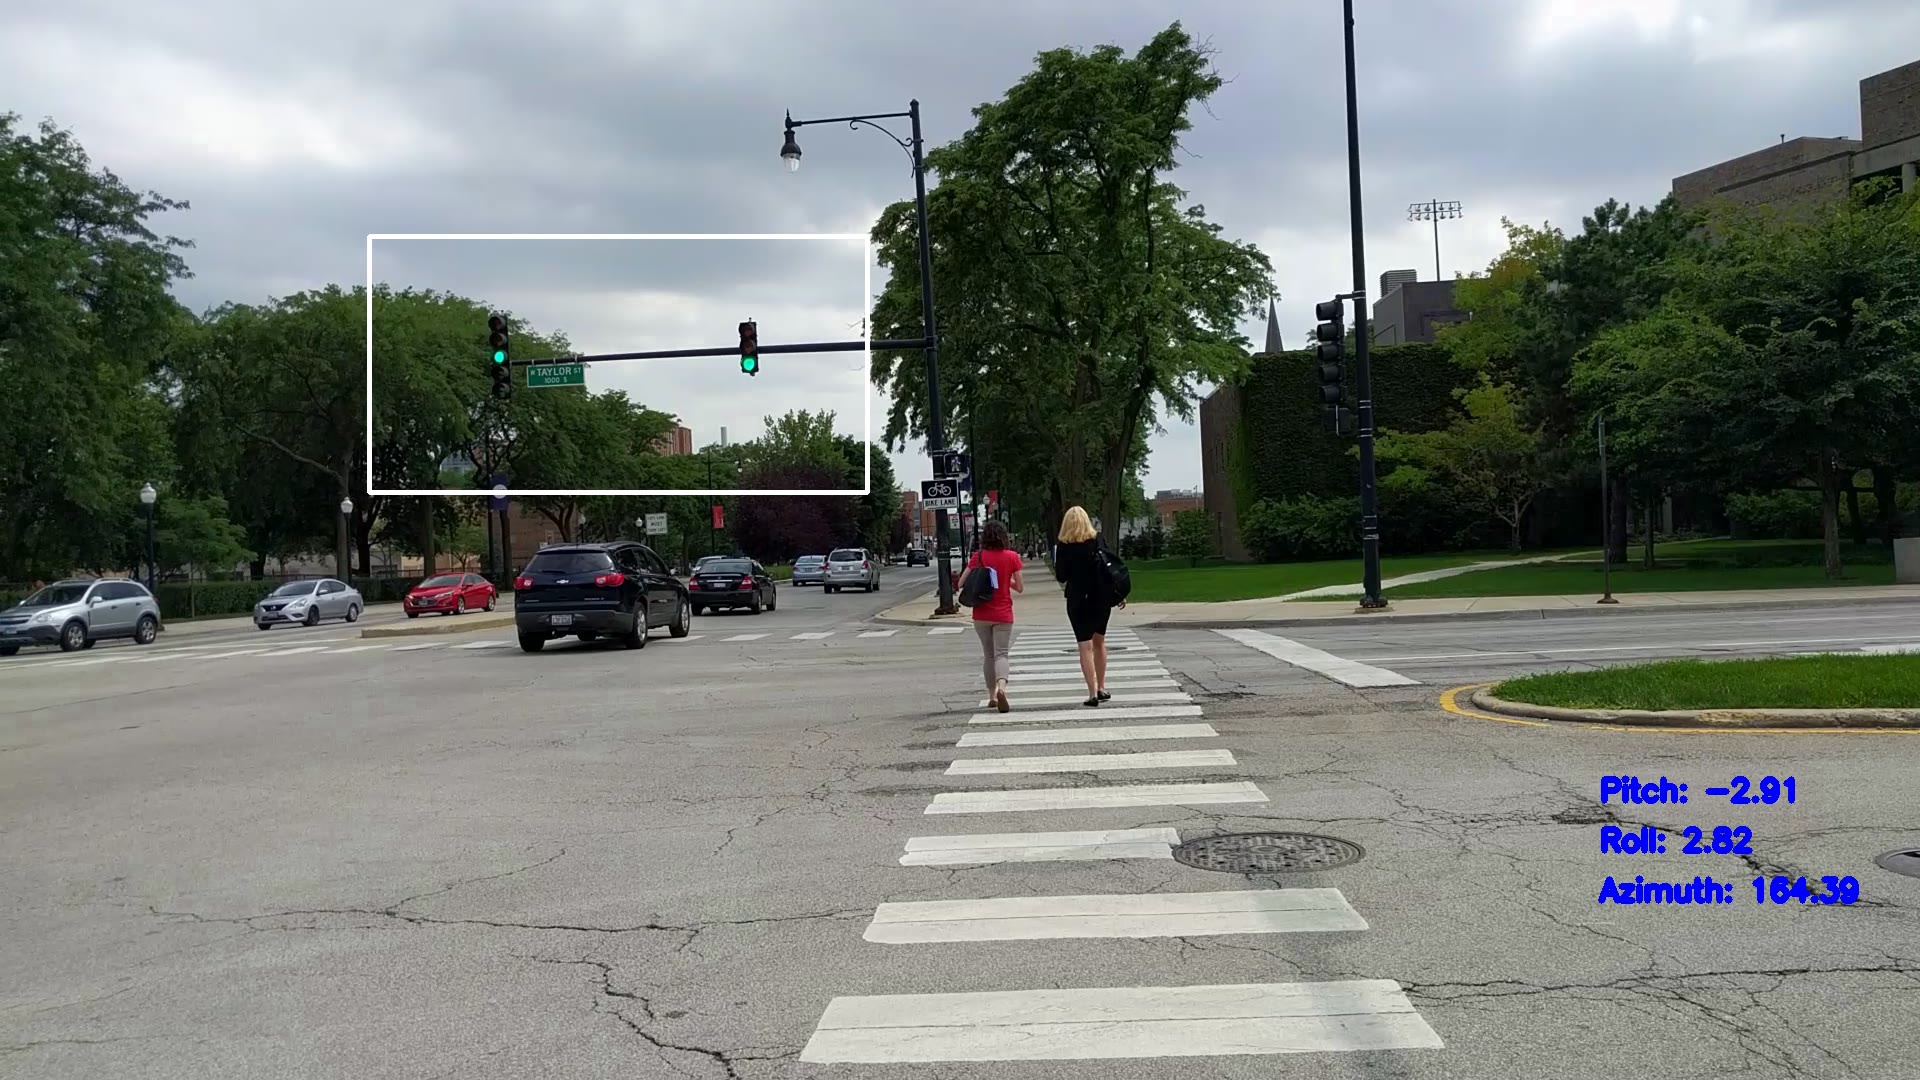
\includegraphics[width=4.2in]{images/rec_mv.jpg}}\\
\subfloat[Movement with change of sensor data] {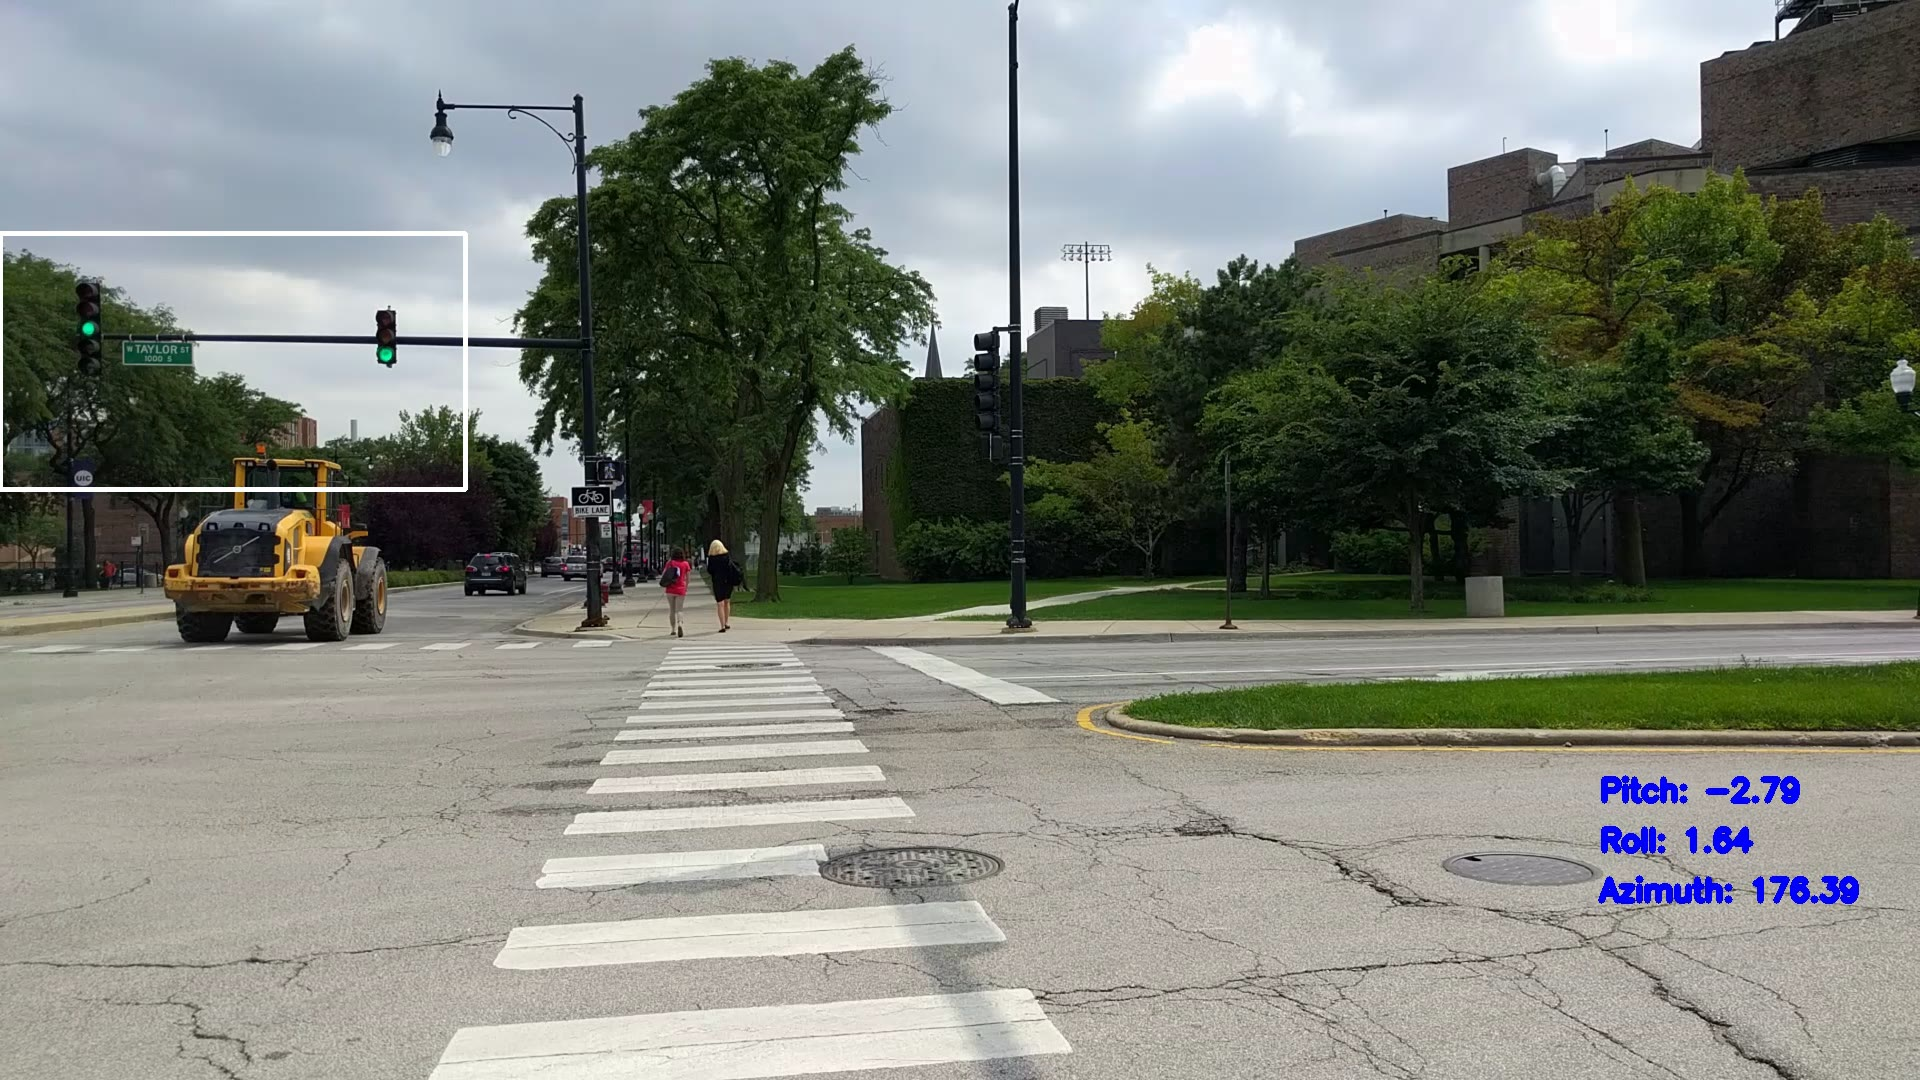
\includegraphics[width=4.2in]{images/rec_mv1.jpg}}\\
\subfloat[Movement with change of sensor data] {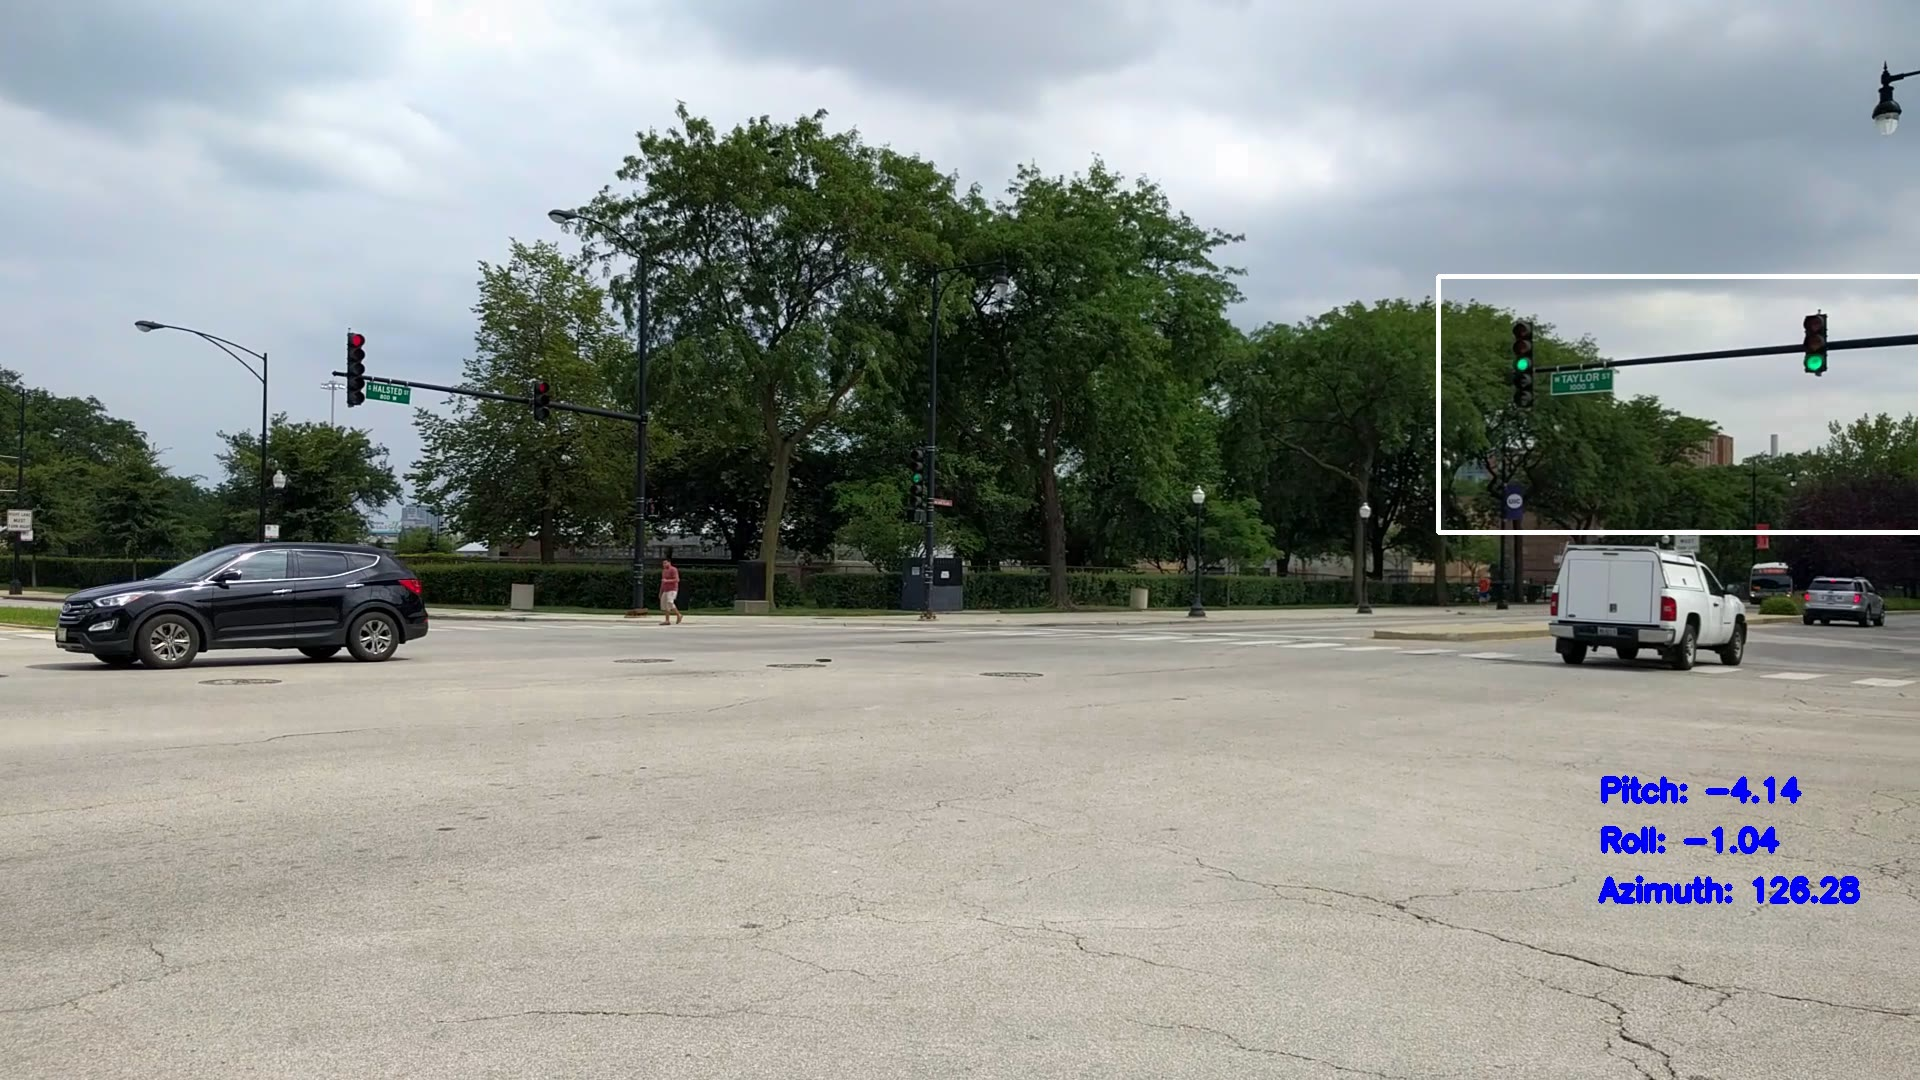
\includegraphics[width=4.2in]{images/rec_mv2.jpg}}

\caption{ROI movement with the change of sensor data.}
\label{f:rec_mv}
\end{figure*}


With the successful detection, our region of interest again changes with the light position and pitch and azimuth value.
For unsuccessful detection, ROI enlarged until it process the full frame and then go to the next frame to detect traffic light.
And this process is continuing to every frame.

\begin{figure*}[!ht]
\centering
\subfloat {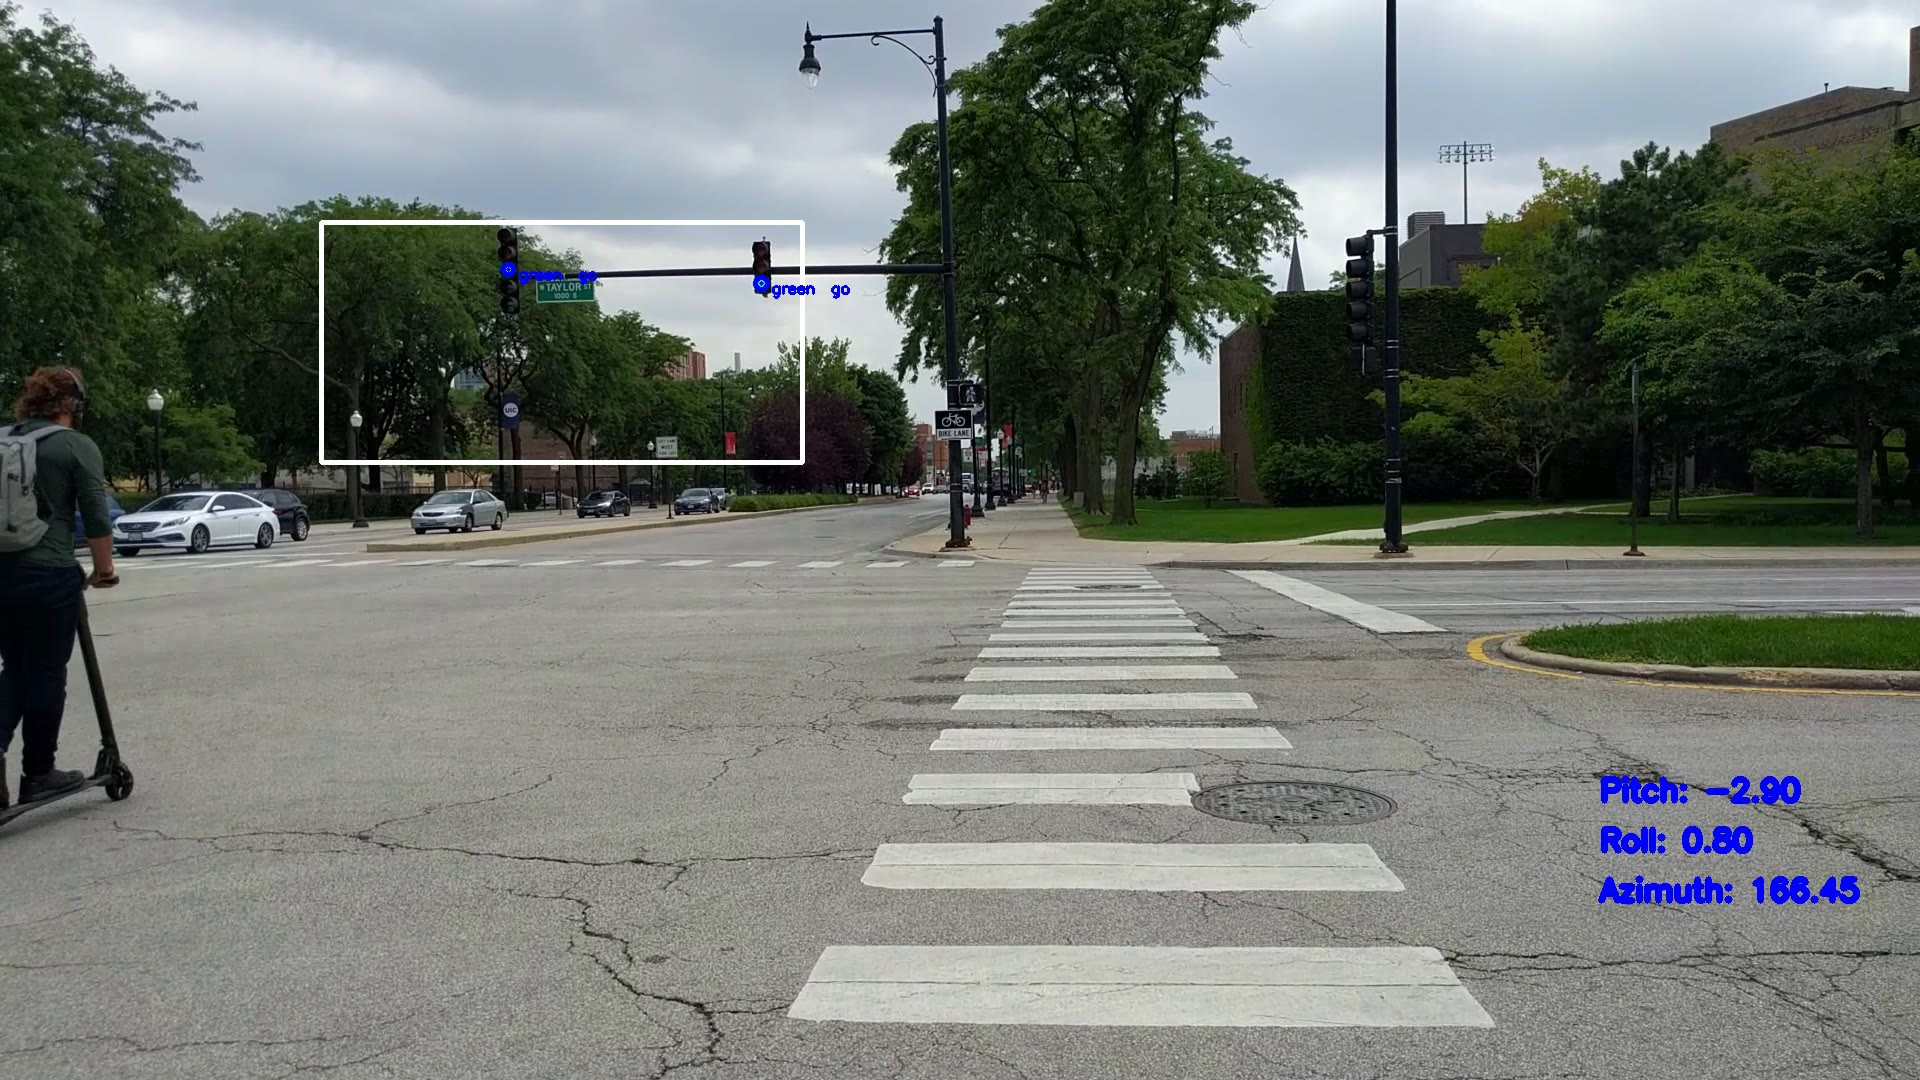
\includegraphics[width=4.2in]{images/rec_enl.jpg}}\\
\subfloat {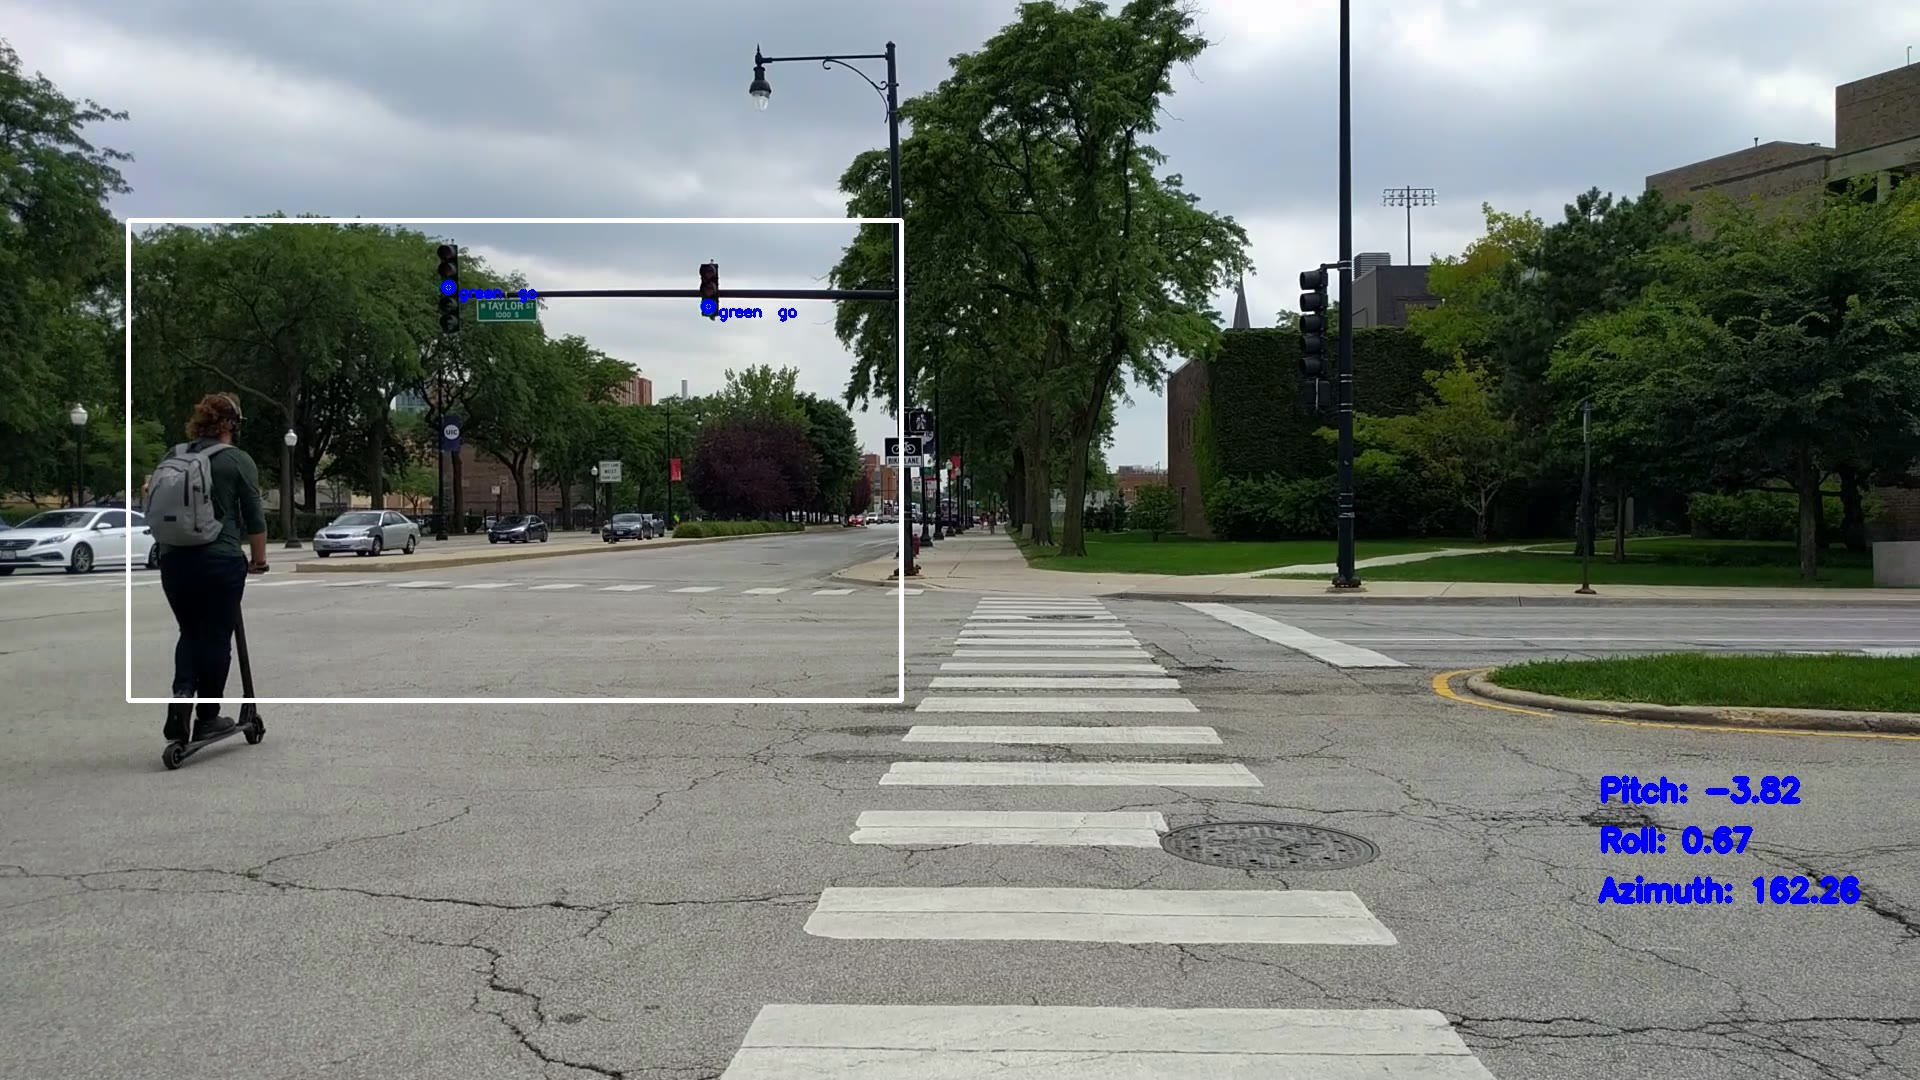
\includegraphics[width=4.2in]{images/rec_enl1.jpg}}

\caption{Enlarged ROI to detect traffic light successfully.}
\label{f:rec_enl}
\end{figure*}


